% ************************** 文档基础配置 **************************
% 文档类：ctexbook（中文书籍专用，基于book类扩展）
% 12pt：字体大小，a4paper：纸张大小，openany：章节可在任意页开始（默认openright仅右页）
\documentclass[12pt,a4paper,openany]{ctexbook}

% 引入常用包（按需增减）
\usepackage{geometry}       % 设置页边距
\usepackage{fancyhdr}       % 自定义页眉页脚
\usepackage{graphicx}       % 插入图片
\usepackage{tabularx}       % 灵活表格
\usepackage{amsmath,amssymb}% 数学公式
\usepackage{bm}
\usepackage{makeidx}        % 生成索引
\usepackage{lipsum}         % 生成测试文本（实际使用时可删除）
\usepackage[style=gb7714-2015]{biblatex} % 参考文献（国标GB/T 7714-2015）
\usepackage[hidelinks]{hyperref}       % 超链接（目录、参考文献跳转）- 移到最后加载避免冲突
\usepackage{xcolor}
\usepackage{xurl}
\usepackage{mhchem}
\graphicspath{{images/}}

\usepackage{caption} % 加载caption宏包，用于配置标题格式
% 全局配置：去掉所有标题的分隔符（冒号），编号与正文之间留空格
\captionsetup{labelsep=space} 

\usepackage{tcolorbox}  % 彩色框核心包
\tcbuselibrary{skins,breakable} % 扩展样式和跨页支持

\newtcolorbox{examplebox}[1][]{% 定义“EXAMPLE”框（蓝色风格）
  colback=white,   % 背景色：蓝色调浅（可调整深浅）
  colframe=blue,            % 边框色：蓝色
  coltitle=white,           % 标题文字色：白色
  fonttitle=\bfseries,      % 标题字体：粗体
  title=例题,            % 默认标题
  #1                        % 允许额外参数（可选）
}

\newtcolorbox{exercisebox}[1][]{% 定义“EXERCISE”框（浅灰风格）
  colback=gray!10!white,    % 背景色：浅灰色
  colframe=gray,            % 边框色：灰色
  coltitle=black,           % 标题文字色：黑色
  fonttitle=\bfseries,      % 标题字体：粗体
  title=EXERCISE,           % 默认标题
  #1                        % 允许额外参数（可选）
}

\usepackage[author={TFAA}, icon=Note, color=red, open=true]{pdfcomment}

% ************************** 页面布局 **************************
% 设置页边距（上3cm，下2.5cm，左3cm，右2.5cm，页眉1.5cm，页脚1cm）
\geometry{
    top=3cm,
    bottom=2.5cm,
    left=3cm,
    right=2.5cm,
    headheight=1.5cm,
    footskip=1cm
}
\parindent=2em          % 首行缩进2字符 

% ************************** 页眉页脚配置 **************************
\pagestyle{fancy}           % 启用自定义页眉页脚
% 清空默认页眉页脚
\fancyhf{}
% 偶数页（左页）：页眉显示书名，页脚显示页码
\fancyhead[LE]{\textbf{\booktitle}}
% 奇数页（右页）：页眉显示章节名（修复：替换未定义的\chaptertitle为\leftmark）
\fancyhead[RO]{\textbf{\leftmark}}
% 所有页脚居中显示页码
\fancyfoot[C]{\thepage}
% 页眉下添加分隔线
\renewcommand{\headrulewidth}{0.4pt}
% 页脚无分隔线
\renewcommand{\footrulewidth}{0pt}

% ************************** 自定义变量（方便修改） **************************
\newcommand{\booktitle}{量子化学}    % 书名
\newcommand{\bookauthor}{Levine}    % 作者
\newcommand{\booktranslator}{TFAA} % 翻译者
\newcommand{\bookdate}{2026年1月}    % 出版日期

% ************************** 参考文献配置 **************************
% 指定参考文献数据库文件（需新建ref.bib文件，放在同目录）
\addbibresource{ref.bib}

% ************************** 索引配置 **************************
\makeindex

% ************************** 正文开始 **************************
\begin{document}

% -------------------------- 封面 --------------------------
% 自定义封面（也可使用\maketitle，按需选择）
\begin{titlepage}
    \centering
    \vspace*{5cm}          % 顶部留白
    {\Huge \bfseries \booktitle \par} % 书名（超大号粗体）
    \vspace{2cm}           % 书名与作者间留白
    {\Large \textit{作者：\bookauthor} \par} % 作者（大号斜体）
    {\Large \textit{译者：\booktranslator} \par}
    \vfill                 % 自动填充空白（推到页底）
    {\large \quad \bookdate \par} % 翻译者+日期
\end{titlepage}

% -------------------------- 扉页/版权页（可选） --------------------------
\newpage
\thispagestyle{empty}      % 隐藏页码
\centering
\vspace*{8cm}
版权所有 © 2026 \bookauthor \\
未经许可，不得复制、转载或摘编 \\
\vfill
\booktranslator \\
\newpage

% -------------------------- 目录 --------------------------
\tableofcontents  % 生成目录
\newpage          % 目录后换页

% -------------------------- 前言/序（可选） --------------------------
\chapter*{前言}   % *表示不编号
\addcontentsline{toc}{chapter}{前言} % 将前言加入目录
\begin{flushleft} % 左对齐
本书适用于化学专业一年级研究生和高年级本科生的量子化学课程。本书为学生提供了量子化学的深入%
讲解，使他们能够理解基本原理。考虑到许多化学专业学生数学基础有限，书中包含了必要的数学知识%
（如复数、微分方程、算子和向量）的复习。推导过程展示详尽，给出每步的细节，以便不同水平的学%
生都能跟上并理解。每章都配有丰富多样的作业题（包括定量题和概念题）。

\vspace{\baselineskip}
第七版新增内容
\vspace{\baselineskip}

第七版做了以下改进：
\begin{itemize}
  \item 全面更新，反映了最新的量子化学研究成果和计算化学方法，包括许多新的文献参考。
  \item 大多数章节都增加了新的习题，包括第 15 章和第 16 章新增的计算题。
  \item 对学生理解有困难的地方进行了修订。
  \item 图表增加了色彩，以增强本书的视觉吸引力。
  \item 《解答手册》和正文中的计算机程序已从 BASIC 语言改为 C++ 语言。
  \item 正文中增添了对量子力学现代研究的引用，例如Ozawa对不确定性原理的重新表述以及对大分子干涉效应的观测。
\end{itemize}

\medskip % 模块之间增加少量空白，排版更美观（可选，贴合书籍格式）

第七版新增和扩充的内容包括：
\begin{itemize}
  \item 不确定性原理的新理论和实验工作（第 5.1 节）。
  \item 计算原子电荷的 CM5 和 Hirshfeld-I 方法（第 15.7 节）。
  \item 静态和动态相关性（第 16.1 节）。
  \item 对完全基组（CBS）极限外推的扩展论述（第 15.5、16.1 和 16.4 节）。
  \item 两电子约化密度矩阵的使用（第 16.2 节）。
  \item DFT-D3 方法（第 16.5 节）。
  \item 用于色散的 vv10 相关泛函（第 16.5 节）。
  \item W1-F12 和 W2-F12 方法（第 16.6 节）。
  \item DNA 中的色散（堆积）相互作用（第 16.8 节）。
  \item MP2.5、MP2.X、SCS(MI)-CCSD 和 SCS(MI)-MP2 方法（第 16.8 节）。
  \item 对核磁共振屏蔽常数和自旋-自旋耦合常数计算的扩展讨论，包括线性缩放（第 16.9 节）。
  \item 片段化方法（第 16.10 节）。
  \item PM6-D3H4 和 PM7 方法（第 17.4 节）。
\end{itemize}

\medskip % 模块之间增加少量空白（可选）
资源：可选的 Spartan 学生版分子建模软件提供了一个先进的分子建模工具包，它将易于使用的图形界面与一组有针对性的计算功能相结合。本书各章末尾问题的答案手册可在 \url{http://www.pearsonhighered.com/advchemistry} 获取。
\end{flushleft}
\newpage
\begin{flushleft}
    \setlength{\parindent}{2em}
量子化学计算在化学各个领域的广泛应用使得所有化学专业的学生都迫切需要掌握现代电子结构计算方法。编写本书的目的就在于此。

我力求使解释清晰完整，不回避难以理解或微妙的要点。推导过程会给出足够的细节以便于理解，而且尽可能避免使用“可以证明……”这种令人沮丧的表述。本书旨在让学生对量子力学和分子电子结构的物理及数学方面有扎实的理解。本书旨在为化学的所有分支领域的学生提供帮助，而不仅仅是为未来的量子化学家服务。然而，这次的讲解内容使得那些继续从事量子化学研究的人能够打下坚实的基础，并且不会因错误观念而受到阻碍。

许多化学专业的学生在学习量子力学时面临的一个难题是他们对所需数学知识的不熟悉。在这篇文章中，我详细阐述了所需的数学知识。我并没有将所有的数学内容放在一个介绍性的章节或一系列附录中，而是将数学与物理学和化学相结合。将数学直接应用于解决量子力学问题，会让学生觉得这些数学知识更有意义，而不是单独学习数学。我还考虑到许多化学专业学生物理学背景有限的情况，因而会回顾物理学的相关内容。

这本书的前几版得益于莱兰·艾伦、N. 科林·贝里德、斯蒂芬·伯纳塞克、詹姆斯·博尔顿、W. 戴维·钱德勒、唐纳德·切斯纳特、R. 理查德·詹姆斯·克罗斯、加里·德博尔、道格拉斯·多伦、大卫·法雷利、梅尔文·费恩伯格、戈登·A. 加拉格、丹尼尔·杰里蒂、大卫·戈德堡、罗伯特·格里芬、特雷西·汉密尔顿等人的评论和建议。莎伦·哈梅斯-席弗、詹姆斯·哈里森、约翰·海德、沃伦·赫赫雷、罗伯特·希恩、汉斯·贾费、米克洛斯·凯特兹、尼尔·凯斯纳、哈里·金、彼得·科尔曼、安娜·克里洛夫、梅尔、莱维、厄罗尔·勒瓦斯、乔尔·利布曼、蒂恩-松·汤姆·林、瑞安·麦克劳克林、弗兰克·米克斯、罗伯特·梅茨格、查尔斯·米尼尔、约翰·H ·摩尔 佩德罗 ·穆伊诺 威廉 ·帕克 莎伦 ·帕尔默 基尔 ·彼得森 加里 ·普费弗 拉塞尔 ·皮泽特 奥列格 ·普雷兹多 弗兰克 ·里乌斯 肯尼思 ·桑多 哈里 ·舒尔 詹姆斯 ·J ·P ·斯图尔特 理查德 ·斯特拉特 傅明 ·陶 罗纳德 ·特里 亚历杭德罗 ·瓦尔谢尔 彼得 ·韦伯 约翰 ·S ·温恩 和 迈克尔 ·泽内尔。

第七版的审稿人有：
\begin{itemize}
\item 约翰·阿斯伯里，宾夕法尼亚州立大学
\item 穆·亨·贝克，印第安纳大学
\item 琳恩·巴奇尔，塔夫茨大学
\item 理查德·达韦斯，密苏里科技大学
\item 卡柳·卡恩，加利福尼亚大学圣巴巴拉分校
\item 斯科特·基尔比，东田纳西州立大学
\item 何塞·莫拉莱斯，德克萨斯技术大学
\item 鲁本·帕拉，德保罗大学
\item 迈克尔·韦德洛克，盖蒂斯堡学院
\end{itemize}

\noindent 我要感谢所有这些人士以及几位匿名审稿人提出的宝贵建议。

我非常希望能收到读者们提出的任何可能改进这本书的建议。
\begin{flushright}
Ira·N·Levine

INLevine@brooklyn.cuny.edu
\end{flushright}
\end{flushleft}
\newpage
\chapter*{译者言}
\addcontentsline{toc}{chapter}{译者言}
\begin{flushleft}
本书于2026年1月28日开始翻译
\end{flushleft}

% -------------------------- 正文章节 --------------------------
\chapter{薛定谔方程}
\section{量子化学}
\begin{flushleft}
    \setlength{\parindent}{2em}
在十七世纪，艾萨克牛顿发现描述宏观物体运动法则的经典力学。在二十世纪早期，物理学家们发现经典力学并不能正确地描述像原子与分子中电子和原子核这样非常微小的粒子。这样粒子的行为被一系列称作\textbf{量子力学}的规律所描述。

\textbf{量子化学}将量子力学应用于化学问题。量子化学的影响在化学的各个分支中都显而易见。物理化学家利用量子力学（借助统计力学）计算气体的热力学性质（例如熵、热容）；解释分子光谱，从而能够通过实验确定分子的性质（例如分子构型、偶极矩、旋转势垒、构象异构体能量差）；从理论上计算分子性质；计算化学反应过渡态的性质，从而能够估算反应速率常数；理解分子间作用力；以及处理固体中的键合问题。

有机化学家利用量子力学来估算分子的相对稳定性，计算反应中间体的性质，研究化学反应的机理，并分析和预测核磁共振谱。

分析化学家广泛使用光谱学方法。只有通过量子力学才能正确理解和解释光谱中谱线的频率和强度。

无机化学家使用配位场理论，这是一种近似的量子力学方法，来预测和解释过渡金属配合离子的性质。

尽管生物重要分子的庞大尺寸使得对其的量子力学计算极其困难，但生物化学家已经开始从对生物分子构象、酶-底物结合以及生物分子溶剂化的量子力学研究中获益。

量子力学决定了纳米材料（至少有一个维度在1至100纳米范围内的物体）的特性，并且正在开发处理纳米材料的计算方法。当材料的一个或多个维度小于100纳米（尤其是小于20纳米）时，其光学、电子、化学及其他性质会与整体材料的性质产生显著差异。尺寸在1至100纳米范围内的半导体或金属物体被称为\textit{量子阱}；有两个维度在这个范围内的就是\textit{量子线}；而所有三个维度均在此范围的则是一个\text{量子点}。这些名称中的量子一词表明量子力学在决定此类材料的特性方面起着关键作用。许多人推测纳米科学和纳米技术将会带来“下一次工业革命”。

计算机运算速度的大幅提升以及新的分子计算方法（如密度泛函理论——第16.4节）的出现，使得量子化学在化学的各个领域都成为了实用的工具。如今，有几家公司出售用于进行分子量子化学计算的量子化学软件。这些程序旨在供各类化学家使用，而不仅仅是量子化学家。由于量子化学及其相关理论和计算方法的作用迅速扩大，美国化学学会于2005年开始出版一份新的期刊，《化学理论与计算杂志》（Chemical Theory and Computation）。 

“量子力学……是现代科学和技术的基础。它控制着晶体管和集成电路的运作……并且……是现代化学和生物学的基础”（Stephen Hawking，\textit{A Brief History of Time}，1988，Bantam，第4章）。
\end{flushleft}
\section{量子力学的历史背景}
\begin{flushleft}
    \setlength{\parindent}{2em}
量子力学的发展始于1900年普朗克对加热固体所发出的光的研究，所以我们先来探讨一下光的本质。

1803年，托马斯·杨通过观察光穿过两个相邻小孔时产生的衍射和干涉现象，为光的波动性提供了令人信服的证据。（衍射是指波绕过障碍物发生弯曲的现象。干涉是指两个频率相同的波相互叠加，在空间的每一点上，其扰动都是由每个波在该点引起的扰动的代数和或矢量和。参见任何一本大学一年级的物理教材。）

1864年，詹姆斯·克拉克·麦克斯韦发表了四条方程，即麦克斯韦方程组，统一了电学和磁学的定律。麦克斯韦方程组预测，加速的电荷会以电磁波的形式辐射能量，这种电磁波由振荡的电场和磁场组成。麦克斯韦方程组所预测的这些波的速度与实验测量的光速相同。麦克斯韦由此得出结论，光是一种电磁波。

1888年，海因里希·赫兹检测到了由电火花中加速电荷产生的无线电波，这与麦克斯韦方程组的预测相符。这使物理学家们确信光确实是一种电磁波。

所有电磁波在真空中的传播速度均为$c=2.998\times 10^8\ \text{m/s}$。其频率$\nu$和波长$\lambda$之间存在如下关系：
\begin{equation}
\boxed{\lambda \nu\ =\ c}
\end{equation}
（被包裹在方框里的方程是需要记忆的。希腊字母表在附录里提供。）电磁波根据其频率有很多传统的名称。无线电波、微波、红外辐射、可见光、紫外辐射、X射线和伽玛射线的频率依次上升。我们应用术语\textbf{光}来描述任一种电磁波。可见光和紫外辐射的波长从前以埃（\AA）表示，而现在以纳米（nm）表示：
\begin{equation}
\boxed{1\ \text{nm}\ =\ 10^{-9}\ \text{m},\quad1\ \AA\ =\ 10^{-10}\ \text{m}\ =\ 0.1\ \text{nm}}
\end{equation}
在十九世纪90年代，物理学家测量了一个确切温度黑体发射的不同频率光的强度，并在不同温度下进行多组测定。\textit{黑体}是指一种吸收所有射向它的光的物体。一种对黑体的良好近似为带有小孔的空腔。在1896年，物理学家Wien提出黑体辐射相对于光频率和黑体温度的公式如下：$I\ =\ a\nu ^3/e^{b\nu /T}$,其中a和b是实验常量，而$I\ \mathrm{d}v$是在频率$\nu$到$\nu\ +\ \mathrm{d}\nu$范围内单位时间单位表面积黑体辐射的能量，$\mathrm{d}\nu$是极小的频率区间。Wien公式对于在1896年可得的黑体辐射数据而言是符合得很好的，但他对该公式的理论论证并不使人满意。

1899-1900年，对于黑体辐射的测量被拓展到较低频率，而在低频率下其数据显示出对Wien公式的明显偏离。这些偏离引导物理学家Max Planck在1900年十月提出一下公式：$I\ =\ a\nu ^3/(e^{b\nu /T}\ -\ 1)$,对所有频率的数据都拟合得很好。

提出这条公式后，Planck为其找到了一种理论解释。1900年12月，他在《德国物理学会》（German Physical Society）展示了他的理论推演。Planck假设黑体中的辐射发射体和吸收体是有规律振荡的电荷（“谐振子”），在空腔中达到电磁辐射平衡。他假定那些频率为$\nu$的谐振子的总能量由N个不可分的“能量单元”构成，每个大小为$h\nu$，其中N是整数而$h$（\textbf{Planck常数}）是一个新的物理学常数。Planck将这些能量单元分配到谐振子中。事实上，这限制每个谐振子的能量是$h\nu$的整数倍（尽管Planck没有明说）。因而每个谐振子的能量是\textbf{量子化}的，表示一个谐振子的能量只能是唯一确定的离散值。Planck的理论推导出$a\ =\ 2\pi h/c^2$，$b\ =\ h/k$，其中$k$是Boltzmann常数。通过对实验黑体曲线的拟合，Planck发现$h\ =\ 6.6\ \times\ 10^{-34}\ \mathrm{J} \cdot \mathrm{s}$。

Planck的工作一般被认为标志着量子力学的诞生。然而物理史学家关于Planck在1900年是将能量量子化作为对物理学的本质还是仅仅作为一种使他获得正确黑体辐射公式的数学近似存在争论。[\textnormal{见O. Darrigol, \textit{Centaurus}, 43, 219 (2001); C. A. Gearhart, \textit{Phys. Perspect.}, 4, 170 (2002)（可在线获取：\url{https://employees.csbsju.edu/cgearhart/Planck/PQH.pdf}）; S. G. Brush, \textit{Am. J. Phys.}, 70, 119 (2002)（\url{https://www.punsterproductions.com/~sciencehistory/cautious.htm}）。}]物理史学家Kragh指出：“如果1900年12月在物理学上发生了一场革命，似乎没有人在当时注意到。Planck也不例外，而人们对他工作的重要性评价很大程度上依赖于历史重构。”（H.Kragh.\textit{Physics World},\ Dec.\ 2000,p.31）

能量量子化的概念与以前所有的物理学观念完全矛盾。根据牛顿力学，一个物体的能量可以连续变化。但只有使用量子化能量的假设才能使人推得正确的黑体辐射曲线。

能量量子化第二次被用在光电效应。在\textit{光电效应}中，光照射在金属上造成电子的发射。一束波的能量与其强度呈正比而与其频率无关，因此光的电磁波图使人预期，一个发射的光电子的动能将随着激发光的强度增加而增加，不随激发光频率的变化而变化。然而相反的，人们观察到光电子的动能与光强度无关却随光的频率增加而增加。

1905年，Einstein提出可以通过将光视作如粒子般的实体（被称为\textbf{光子}），且每个光子具有符合以下公式的能量来解释观察到的现象。
\begin{equation}
\boxed{E_{\text{photon}}\ = \ h\nu}
\end{equation}
当金属中的一个电子吸收一个光子，一部分光子能量被用于克服金属对电子的束缚力；剩余部分表现为电子离开金属后的动能。能量守恒给出$h\nu\ =\ \Phi\ +\ T$，其中$\Phi$是一个电子脱离金属所需的最小能量（金属的\textit{逸出功}），$T$是发射电子的最大动能。激发光的频率$\nu$增加提高光子的能量，因此增大发射电子的动能。当频率固定时激发光强度的增加增大光子撞击金属的速率，因而增大电子发射的速率，但并不改变每个发射电子的动能。（根据Kragh所说，有充分的“理由可以证明，是爱因斯坦首先认识到了量子理论的精髓”；Kragh,\textit{Physics World, Dec. 2000, p.31.}）

光电效应表明光除了在衍射实验实验中展现的波行为外，也可以展现出粒子行为。

1907年，Einstein将能量量子化应用于固体元素中原子的振动，假定每个原子在每个方向$(x,y,z)$上的振动能量只能是$h\nu_{vib}$的整数倍，其中振动频率$\nu_{vib}$是该元素的特性。利用统计力学，Einstein推导了固体恒容热容$C_V$的表达式。Einstein的方程同已知金刚石的$C_V$-温度数据吻合得相当好。

我们现在来考虑物质的结构。

在十九世纪，对放电管和自然放射现象的研究表明原子和分子由带电粒子组成。电子带有一个负电荷。质子带有一个与电子电量相等但电性相反的正电荷且要比电子重1836倍。原子的第三种组成中子（1932年发现），不带电荷且略重于质子。

从1909年开始，Rutherford，Geiger和Marsden重复用一束$\alpha$粒子轰击金属薄箔，观察到落在荧光屏上的粒子出现偏转。$\alpha$粒子是由自然放射衰变得到的带正电荷的氦核。大部分$\alpha$粒子基本未偏转地穿过金属箔，但令人惊奇的是，一些粒子发生了大角度偏转，有些甚至偏转而返回。为了获得大角度的偏转，一个$\alpha$粒子的轨迹要非常接近电荷，以至于产生巨大的库伦排斥。如果正电荷分布于整个原子（如J.J.Thomson在1904年提出的那样），当高能$\alpha$粒子穿入原子，根据经典静电学，库伦排斥将减弱，在原子中心处达到0。因此Rutherford得出结论，如此大的偏转仅可能在电荷集中在一个体积微小、质量极大的核时发生。

一个原子有一个微小（半径$10^{-15}$到$10^{-12}\ $cm）、质量很大的由中子与Z个质子组成，其中Z是原子序数。在原子核外是Z个电子。带电荷的粒子间作用遵循库伦定律。（核子通过强而短程的核力束缚在一起，我们在这无需关心。）一个原子的半径在1埃左右，比如气体动力学理论便证明了这一点。分子含有不少于一个原子核。

原子和分子的化学性质由他们的电子结构决定，所以问题来到电子运动和能量的本质。因为原子核要远重于电子，我们预期核的运动较电子运动而言是微不足道的。

1911年，Rutherford提出他的原子行星模型，其中电子围绕原子核在不同的轨道旋转，就像行星围绕太阳一样。然而，该模型有一个根本性的难题。根据经典电磁学理论，一个加速的带电粒子会以电磁（光）波的形式辐射能量。一个围绕核以恒定速率旋转的电子是被加速的，因为它速度矢量的方向持续地改变。因此Rutherford模型中的电子应当持续地通过辐射失去能量，因而将旋转落入原子核中。所以，根据经典（十九世纪）物理，RutherFord原子是不稳定的，必将坍缩。

Niels Bohr在1913年提出一种可能的摆脱此难题的方法，他将能量量子化的概念应用于氢原子。Bohr假设一个氢原子中电子的能量是量子化的，电子被限制在大量允许的圆周之一上运动。当一个电子从一个Bohr轨道上跃迁到另一轨道，一个频率$\nu$满足关系
\begin{equation}
\boxed{E_{upper}\ -\ E_{lower}\ =\ h\nu}
\label{eq1.4}
\end{equation}
的光子被吸收或释放，其中$E_{upper}\text{和}E_{lower}$是较高能级和较低能级的能量（能量守恒）。根据一个从自由（电离）态跃迁到束缚态的电子释放出一个光子，其频率为束缚轨道中电子公转的经典频率一半的整数倍的假定，Bohr利用经典力学推导出氢原子能级的公式。利用式\eqref{eq1.4}，他的推论与氢原子光谱相符合。但是使用Bohr理论不能拟合氦原子光谱。此外，这套理论无法解释分子中的化学键。

Bohr模型的失败来源于用经典力学去描述原子中的电子运动。原子光谱表现出分立频率的事实，暗示只有特定的运动能量是被允许的；电子能量是量子化的。然而，经典力学允许连续的能量。量子化出现在波的运动中——例如，小提琴的基频、泛音的频率。因此Louis de Broglie在1923年提出电子的运动也许具有波的性质；电子的质量$m$和速度$v$满足波长
\begin{equation}
\lambda\ =\ \frac{h}{mv}\ =\ \frac{h}{p}
\label{De Broglie公式}
\end{equation}
其中$p$是线动量。De Broglie通过合理类比光子推得公式\eqref{De Broglie公式}。根据Einstein狭义相对论，光子的能量可以被表示为$E\ =\ pc$其中$c$是光速，$p$是光子的动量。对一个以光速运动的光子，利用公式$E_{photon}\ =\ h\nu$，我们可以得到$pc\ =\ h\nu\ =\ \frac{hc}{\lambda}$即$\lambda\ =\ \frac{h}{p}$。公式\eqref{De Broglie公式}则是相应对于电子的方程。

1927年，Davisson和Germer通过令电子在金属表面反射并观测到衍射现象，在实验上证实了de Broglie的假说。1932年，Stern用氦原子和氢分子观察到了相同的现象，从而证实波动性并非只是电子的特性，而是对于微观粒子的某种普遍的运动规律。像\ce{C48H26F24N8O8}这样大的分子在穿过一个衍射光栅时都能观测到衍射和干涉[T. Juffmann et al., Nat.Nanotechnol., 7, 297 (2012).]一个包含\ce{C32H18N8}分子干涉图样形成的视频可以在\url{www.youtube.com/watch?v=vCiOMQIRU7I}上观看。

综上所述电子在某些方面表现的像粒子而某些方面像波。我们遇到一种物质（以及光）明显矛盾的的“波粒二象性”。电子怎么能既是波，一种定域的实体，又是非定域的波？答案是一个电子既不是波也不是粒子，而是一种其他的存在形式。不可能用经典物理中波或粒子的概念去精准描述粒子的行为图景。经典物理观念从宏观世界的经验中发展而来，并不能很好地描述微观世界。进化使得人类大脑充分地理解和处理宏观现象。人类的神经系统却没有发展到处理原子和分子级别的现象，因此我们无法完全理解这样的现象并不令人惊讶。

尽管光子和电子都展示出明显的二象性，它们并不是相同种类的实体。光子在真空中以光速$c$运动且静止质量为零；电子的速度$v$总是小于$c$且其静止质量非零。光子总是要考虑其相对论效应，但速度远小于$c$的电子可以在非相对论情况下处理。
\end{flushleft}
\section{不确定原理}
\begin{flushleft}
    \setlength{\parindent}{2em}
让我们考虑波粒二象性对同时测量一个微观粒子的$x$坐标和线动量的$x$方向分量尝试的影响。我们从一束动量为$p$、向$y$方向运动的粒子，且让这束粒子通过一条狭缝。在狭缝后是照相底片。见图\eqref{pic1.1}。
\begin{figure}[bhtp]
    \centering % 图片居中显示（核心命令）
    % 插入图片并调整大小：width=0.8\textwidth 表示图片宽度为页面宽度的80%
    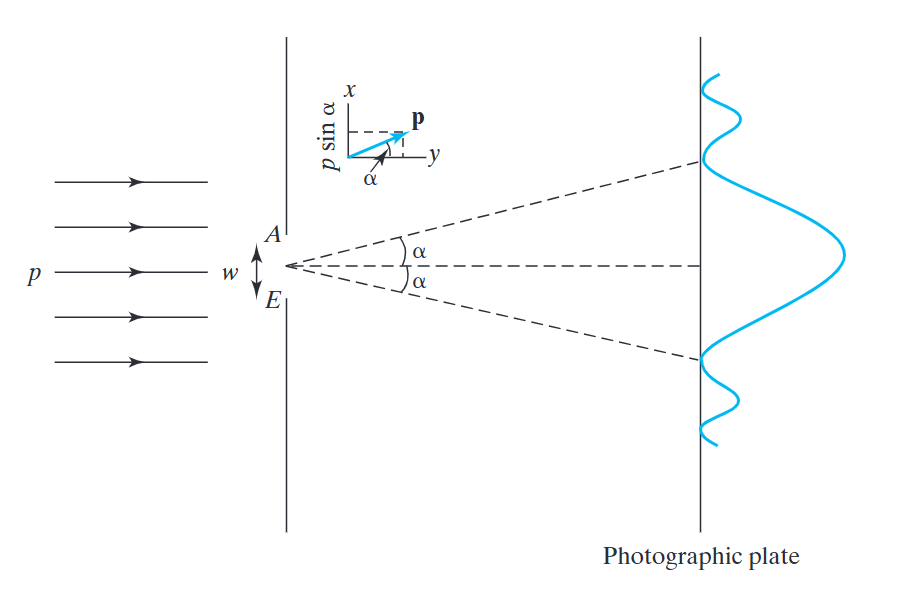
\includegraphics[width=0.8\textwidth]{1.1}
    % 图片标题（会自动生成编号，如Figure 1）
    \caption{电子狭缝衍射}
    % 图片引用标签（后续可通过\ref{pic1}引用图片编号，必须放在\caption之后）
    \label{pic1.1}
\end{figure}

穿过宽度为$w$狭缝的粒子在其穿过狭缝时在$x$坐标上有不确定度$w$。把这段在$x$上的展宽叫做$\Delta x$，有$\Delta x\ =\ w$。

因为微观粒子具有波的性质，它们通过狭缝发生衍射，在底片上产生（就像光束）衍射图样。图\eqref{pic1.1}中曲线的高度表示测量到的到达底片某一点处粒子的数量。衍射图样表明当粒子通过狭缝发生衍射时，它们运动的方向发生改变，因而部分动量被转移到$x$方向上。$x$方向上动量分量$p_x$等于动量矢量$\mathbf{p}$在$x$方向上的投影。一个向上偏转角度为$\alpha$的粒子的$x$方向动量分量$p_x\ =\ p\sin \alpha$，向下偏转角度为$\alpha$的粒子的$x$方向动量分量$p_x\ =\ -p\sin \alpha$。因大部分粒子偏转角度在$-\alpha$到$\alpha$，其中$\alpha$是衍射图样中第一个极小值对应的角度，我们选取中央衍射峰里动量展宽的一半作为动量在$x$方向分量的不确定度$\Delta p_x$的测量值：$\Delta p_x\ =\ p\sin\alpha$。

因此在进行测量的狭缝处，
\begin{equation}
    \Delta x\Delta p_x\ =\ pw\sin\alpha
    \label{uncertainty}
\end{equation}
\begin{figure}[hbtp]
    \centering
    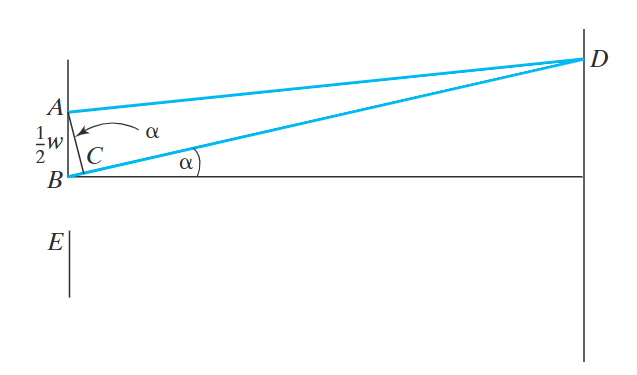
\includegraphics[width=0.8\textwidth]{1.2}
    \caption{一级最小衍射角计算}
    \label{pic1.2}
\end{figure}

在一级最小衍射值处的角度$\alpha$已经计算得到。一级极小的条件是从狭缝上端通过的粒子和从中间通过的粒子飞行距离差等于$\frac{1}{2}\lambda$，其中$\lambda$是相关波的波长。从狭缝上端发出的波与从中间发出的波相位完全相反，因而它们干涉相消。从一个比狭缝中心低$d$的点发出的波与从比狭缝顶点低$d$的点发出的波干涉相消。在图\eqref{pic1.2}中作AC使得$AD\ =\ CD$，有$BC$为路程差。从狭缝到光屏的距离相较狭缝的宽度而言很大。因而$AD$和$CD$几近平行。这导致$\angle ACB$基本是一个直角，所以$\angle BAC\ =\ \alpha$。因此路程差$BC$为$\frac{1}{2}w\sin \alpha$。令$BC$等于$\frac{1}{2}\lambda$，我们有$w\sin \alpha\ =\ \lambda$，公式\eqref{uncertainty}变为$\Delta x\Delta p_x\ =\ h$。因为没有精准定义不确定度，该等号并不合理。相反的我们写
\begin{equation}
    \Delta x\Delta p_x\ \approx\ h
    \label{uncertainty2}
\end{equation}
表示$x$和$p_x$中不确定性的乘积是Planck常数的数量级。

尽管我们在展示公式\eqref{uncertainty2}时只做了一组实验的设置，其实用性是普遍的。无论做了任何尝试，微观“粒子”的波粒二象性对我们同时测量粒子的位置和动量的能力作出限制。我们测量的位置越精确，则测量到的动量越不准确。（在图\eqref{pic1.1}中，$\sin \alpha\ =\ \lambda/w$，因此减小狭缝的宽度将增加衍射图样的展宽。）这种限制就是\textbf{不确定原理}，Werner Heisenberg在1927年发现。

因为波粒二象性，测量的行为会在正被测量的系统中引入不可控的干扰。开始时我们有具有精确$p_x$值（零）的粒子。通过设置狭缝，我们测量到粒子精确的$x$坐标$w$，但这种测量将不确定性引入粒子的$p_x$值。测量会改变系统的状态。\pdfcomment{究竟是测量引起还是物质的内禀性质？}
\end{flushleft}
\section{含时薛定谔方程}
\begin{flushleft}
    \setlength{\parindent}{2em}
经典力学只适用于宏观粒子。对于微观“粒子”，我们需要一种新的力学形式，被称为\textbf{量子力学}。现在我们来考虑经典力学和量子力学之间的一些对比。为了简化，我们将讨论单粒子单维度系统。

在经典力学中，粒子的运动遵从Newton第二定律：
\begin{equation}
    \boxed{F\ =\ ma\ =\ m\frac{\mathrm{d}^2x}{\mathrm{d}t^2}}
    \label{N2}
\end{equation}
其中$F$是作用于粒子上的力，$m$是粒子质量，$t$是时间；$a$是加速度，通过公式$a\ =\ \mathrm{d}v/\mathrm{d}t\ =\ (\mathrm{d}/\mathrm{d}t)(\mathrm{d}x/\mathrm{d}t)\ =\ \mathrm{d}^2x/\mathrm{d}t^2$，其中$v$是速度。\eqref{N2}包含坐标$x$对时间的二阶导数。为了处理它，我们需要进行两次积分。这将引入两个任意常数$c_1$和$c_2$，有两个维度在这个范围内的就是
\begin{equation}
    x\ =\ g(t,c_1,c_2)
    \label{eq1.9}
\end{equation}
其中$g$是时间的函数。我们现在要问：我们在一个给定的时间$t_0$时需要什么信息才能预测该粒子未来的运动？如果我们知道在$t_0$时粒子位于$x_0$处，我们有
\begin{equation}
    x_0\ =\ g(t_0,c_1,c_2)
    \label{eq1.10}
\end{equation}
因为我们有两个常数待定，所以需要更多的信息。对式\eqref{eq1.9}微分，我们可以得到
\begin{equation*}
    \frac{\mathrm{d}x}{\mathrm{d}t}\ =\ v\ =\ \frac{\mathrm{d}}{\mathrm{d}t}g(t,c_1,c_2)
\end{equation*}
若我们也知道$t_0$时刻粒子的速度$v_0$，我们就有另外的关系
\begin{equation}
    v_0\ =\ \left. \frac{\mathrm{d}}{\mathrm{d}t}g(t,c_1,c_2)\right|_{t=t_0}
    \label{eq1.11}
\end{equation}
随后我们可能可用\eqref{eq1.10}和\eqref{eq1.11}在已知$x_0$和$v_0$的情况下解出$c_1$与$c_2$。知道了$c_1$与$c_2$，我们便可用公式\eqref{eq1.9}去确切地预测粒子未来的运动。

作为公式\eqref{N2}到公式\eqref{eq1.11}的使用案例，考虑一个粒子在地球重力场中的竖直运动。令$x$轴竖直向上。粒子所受到的重力竖直向下且$F\ =\ -mg$，其中$g$是重力加速度常数。则Newton第二定律\eqref{N2}为$-mg\ =\ m\mathrm{d}^2x/\mathrm{d}t^2$，所以$\mathrm{d}^2x/\mathrm{d}t^2\ =\ -g$。简单的积分便可得到$\mathrm{d}x/\mathrm{d}t\ =\ -gt\ +\ c_1$。若知道时间$t_0$时粒子的速度$v_0$则可确定任意的常数$c_1$。因为$v\ =\ \mathrm{d}x/\mathrm{d}t$，我们有$v_0\ =\ -gt_0\ +\ c_1$即$c_1\ =\ v_0\ +\ gt_0$。因此，$\mathrm{d}x/\mathrm{d}t\ =\ -gt\ +\ gt_0\ +\ v_0$。第二次积分时我们引入另一任意常数$c_2$，其在我们知道$t_0$时刻的位置$x_0$时可计算得到。我们发现（问题1.7）$x\ =\ x_0\ -\ \frac{1}{2}g(t-t_0)^2\ +\ v_0(t-t_0)$。知道$t_0$时刻的$x_0$和$v_0$，我们便可以预测粒子未来的位置。

经典力学中一个粒子在一个维度上运动的势能$V$被定义为满足
\begin{equation}
    \boxed{\frac{\partial V(x,t)}{\partial{x}}\ =\ -F(x,t)}
    \label{eq1.12}
\end{equation}
例如，对于一个在地球重力场中运动的粒子，$\partial V/\partial x\ =\ -F\ =\ mg$，积分得到$V\ =\ mgx\ +\ c$，其中$c$是任意常数。我们可以随意地去设置零势能基准在我们想要之处。选取$c\ =\ 0$，我们有$V\ =\ mgx$作为势函数。

\textbf{状态（state）}一词在经典力学中指在某一时刻对系统中每个粒子的位置与速度的具体描述，加上作用在粒子上的力的具体描述。根据Newton第二定律，给定任一时刻一个系统的状态，其未来的状态和运动都已确定，如公式\eqref{eq1.9}-\eqref{eq1.11}所展示。Newton定律在解释行星运动上令人赞叹的成功导致很多哲学家使用Newton定律作为哲学决定论的论据。数学家和天文学家Laplace（1749-1827）假定全宇宙完全由遵从Newton定律的粒子构成。因此，给定宇宙在某一瞬间的状态，宇宙中任何事物未来的运动都完全确定。从原理上讲，一个知晓宇宙在任一时刻状态的超观测者可以计算所有未来的运动。
\begin{quote}
\small
尽管经典力学是决定论的，很多经典力学系统（比如，在重力、摩擦力和一个周期性变化的驱动力作用下振荡的摆）在特定范围的系统参数下展现出混沌行为。在一个混沌系统中，运动对于粒子位置、速度与受到作用力的初始值非常敏感，两个仅差实验难以探测的量的初始状态，最终将导致系统未来截然不同的行为。因此，因为人可以测得初始状态的准确程度是有限的，对于混沌经典力学系统长期行为的预测在实际上是不可能的，就算系统遵从确定性方程。对于太阳系行星轨道数千万年的计算机计算表明行星运动是混沌的。[I. Peterson, \textit{Newton’s Clock: Chaos in the Solar System}, Freeman, 1993;J. J. Lissauer, \textit{Rev. Mod. Phys.}, \textbf{71}, 835 (1999)].
\end{quote}

给定一个经典力学系统当前状态，我们可以预测其未来的状态。然而，Heisenberg不确定原理表明我们不能同时确定一个微观粒子的位置和速度，所以经典力学预测一个系统未来运动所需的认知本身就无法获得。我们要对量子力学无法完全预测未来精准运动状态之处知足。

我们研究量子力学的方法将为\textit{假定}一些基本公设，再用这些假定去推断实验可测的结果，比如说原子的能级。为了在量子力学中描述一个系统的\textbf{状态}，我们假定一个粒子坐标的函数$\mathbf{\Psi}$存在，成为\textbf{状态函数}或\textbf{波函数}（更多的写作\textbf{波函数}）。因为一般来说状态会随时间改变，$\bm{\Psi}$也是时间的函数。对于单粒子单维度系统，我们有$\bm{\Psi}\ =\ \bm{\Psi}(x,t)$。波函数含有关于一个系统所有的可能的信息，所以我们简单地说“状态$\bm{\Psi}$”而不是称“被波函数$\bm{\Psi}$描述的状态”。Newton第二定律告诉我们如何从一个经典力学系统当前状态找到未来状态。为了从当前状态找到量子力学系统的未来状态，我们想要一条告诉我们波函数如何随时间改变的方程。对于一个单粒子单维度系统，这条方程被假定为
\begin{equation}
    -\frac{\hbar}{i}\frac{\partial\bm{\Psi}(x,t)}{\partial t}\ =\ -\frac{\hbar^2}{2m}\frac{\partial^2\bm{\Psi}(x,t)}{\partial x^2}\ +\ V(x,t)\bm{\Psi}(x,t)
    \label{eq1.13}
\end{equation}
其中常数$\hbar$（约化普朗克常数）被定义为
\begin{equation}
    \boxed{\hbar\ \equiv\ \frac{h}{2\pi}}
\end{equation}
波函数的概念和掌管其随时间的变化的方程在1926年由奥地利物理学家Erwin Schr\"odinger（1887-1961）。在这条被称为\textbf{含时薛定谔方程}（或\textbf{薛定谔波动方程}）的方程中，$i\ =\ \sqrt{-1}$，$m$是粒子的质量，$V(x,t)$是系统的势函数。（很多历史上重要的量子力学论文均可于\url{dieumsnh.qfb.umich.mx/archivoshistoricosmq}获得。）

含时薛定谔方程包含波函数对时间的一阶导数，让我们在知道$t_0$时刻波函数的情况下可以计算未来任一时刻的波函数（状态）。

波函数具有关于其描述的系统我们可能知道的全部信息。$\bm{\Psi}$能给我们对于粒子$x$坐标的测量结果的什么信息？我们不可能期待$\bm{\Psi}$像经典力学系统状态那样包含位置的确切信息。在Schr\"odinger发现薛定谔方程不久后Max\ Born给出此问题正确的答案。Born假设对于一个单粒子单维度系统，
\begin{equation}
    \boxed{\left|\bm{\Psi}(x,t)\right|^2\mathrm{d}x}
    \label{eq1.15}
\end{equation}
给出了$t$时刻在$x$轴的$x$到$x\ +\ \mathrm{d}x$之间找到该粒子的\textit{概率}。在\eqref{eq1.15}中竖线代表绝对值，$\mathrm{d}x$代表$x$轴上一个无限小的长度。函数$\left|\bm{\Psi}(x,t)\right|^2$是在$x$轴不同地方找到粒子的\textbf{概率密度}。（概率将在1.6节中回顾）比如，考虑在某个具体时刻$t_0$粒子处于一个被波函数$ae^{-bx^2}$，其中$a$与$b$是实际的常数。如果我们在$t_0$时刻测量粒子的位置，我们将可能得到任何$x$的值，因为概率密度$a^2e^{-2\cdot bx^2}$在所有地方都不为零。在$x\ =\ 0$附近区域$x$的值比其他地方的值更易被测量到，因为$\left|\bm{\Psi}\right|^2$在此案例中在原点处取最大值。

为了将$\left|\bm{\Psi}\right|^2$与实验测量联系起来，我们将选用很多相同的无互相作用的系统，每个系统有相同的状态$\bm{\Psi}$。随后在每个系统中测量粒子的位置。如果我们有$n$个系统并进行了$n$次测量，且$\mathrm{d}n_x$指我们发现粒子位于$x$到$x\ +\ \mathrm{d}x$之间的测量的次数，则$\mathrm{d}n_x/n$为发现粒子位于$x$到$x\ +\ \mathrm{d}x$之间的概率。因而
\begin{equation*}
    \frac{\mathrm{d}n_x}{n}\ =\ \left|\bm{\Psi}\right|^2\mathrm{d}x
\end{equation*}
$x$对$(1/n)\mathrm{d}n_x/\mathrm{d}x$作图给出概率密度$\left|\bm{\Psi}\right|^2$作为$x$的函数。似乎我们可以通过选择一个处于$\bm{\Psi}$状态的系统并重复地测量粒子位置来获得概率密度函数。这个流程是错误的，因为测量的操作一般会改变系统的状态。在不确定原理的讨论（1.3小节）中我们看到这一现象。

量子力学从本质上来说是\textit{统计的}。已知状态，我们不能确定地预测一次位置测量的结果；我们只能预测各种可能结果的\textit{概率}。Bohr氢原子理论确定了电子的精确运动轨迹，因此不是一个正确的量子力学图景。

量子力学并没有说一个电子像波一样分布在一大片空间里。确切的说，它是用于描述像波一样且满足波动方程的电子运动的概率图样（波函数）。

波函数如何告诉我们除了位置外其他性质的信息将在后续章节中讨论。

热力学的公设（热力学第一、第二、第三定律）是从宏观经验角度陈述的，因而相当容易理解。而量子力学的公设是从微观世界的角度陈述的，显得很抽象。你在第一次读到时不必希望去完全理解量子力学公设。随着我们处理各种例子，你对这些公设的理解会逐渐加深。

我们先写下薛定谔方程而丝毫不去证明其合理性或许会使读者感到困扰。通过几何光学、经典力学与波动光学、量子力学之间的类比，可以说明薛定谔方程的合理性。几何光学是对波动光学的近似，当光的波长远小于仪器尺寸时成立。（回想它用来处理透镜和镜面）。相似的，经典力学也是波动力学的近似，当粒子的波长远小于仪器尺寸时适用。基于几何光学和波动光学之间已知的关系，对于如何从经典力学中得到合理的量子力学方程，我们可以做一个合理猜测。因为很多化学家对于光学尤其得不熟悉，这些论证被省略了。在任何例子中，这样的类比只能让薛定谔方程看起来\textit{讲得通}。它们无法被用于\textit{推演}或\textit{证明}这条方程。薛定谔方程是这套理论的一条\textit{公设}，被其所得预测与实验之间的吻合程度检验。（引导Schr\"odinger得出其方程的推理细节见\textit{Jammer}, Section 5.3.A reference with the author’s name italicized is listed in the Bibliography）

量子力学提供了微观粒子运动的法则。实验上，宏观物体遵从经典力学。因此量子力学要成为有效的理论，当粒子从微观向宏观过渡时它要退化为经典力学。量子效应与de Broglie波长$\lambda\ =\ h/m\nu$相关联。因为$h$非常小，宏观物体的de Broglie波长基本上为零。因此，在极限$\lambda\ \to\ 0$时，我们期望含时薛定谔方程退化为Newton第二定律。可以证明确实如此（见问题7.59）

狭义相对论与经典力学间的关系也是相似的情况。当极限$v/c\ \to\ 0$时（$c$为光速），狭义相对论退化为经典力学。接下来我们推导的量子力学形式将是非相对论的。相对论同量子力学完全的融合还没有实现。

历史上，在Schr\"odinger1926年得到其微分方程数月前，Heisenberg、Born、Jordan在1925年用矩阵第一次确立了量子力学。Schr\"odinger证明了Heisenberg形式（称为\textbf{矩阵力学}）与薛定谔形式（称为\textbf{波动力学}）等价。在1926年，Dirac和Jordan，分别用一种被称为\textit{变换理论（transformation theory）}的抽象形式表述量子力学，该理论是矩阵力学和波动力学的统一（见\textit{Dirac}）。1948年，Feynman提出量子力学的\textit{路径积分（path integral）}形式。 [R. P. Feynman, \textit{Rev. Mod. Phys.}, \textbf{20}, 367 (1948); R. P. Feynman and A. R. Hibbs, \textit{Quantum Mechanics and Path Integrals}, McGraw-Hill, 1965]
\end{flushleft}
\section{定态薛定谔方程}
\begin{flushleft}
    \setlength{\parindent}{2em}
含时薛定谔方程\eqref{eq1.13}看起来很吓人。幸运的是，很多量子力学在化学上的应用并不使用这条方程。相反的，使用更简单的定态薛定谔方程。我们现在在单粒子单维度案例中从含时薛定谔方程推导定态薛定谔方程。

我们从一个特殊的案例开始，其中势函数$V$不是时间的函数，只依赖于$x$。当系统没有受到与时间有关的外部作用力时这是成立的。含时薛定谔方程为
\begin{equation}
    -\frac{\hbar}{i}\frac{\partial\bm{\Psi}(x,t)}{\partial t}\ =\ -\frac{\hbar^2}{2m}\frac{\partial^2\bm{\Psi}(x,t)}{\partial x^2}\ +\ V(x)\bm{\Psi}(x,t)
    \label{eq1.16}
\end{equation}
现在我们限定研究范围，寻找可以作为\eqref{eq1.16}的被写作时间的函数与$x$的函数成绩的解：
\begin{equation}
    \boxed{\bm{\Psi}(x,t)\ =\ f(t)\psi (x)}
    \label{eq1.17}
\end{equation}
大写的psi被用于含时薛定谔方程而小写的psi用于只依赖于坐标$x$的因子。\eqref{eq1.17}形式波函数对应的状态拥有让它们备受关注的确切性质（简要来说）。[并不是所有\eqref{eq1.16}的解都具有\eqref{1.17}的形式；见问题3.51\pdfcomment{去耦合只是取巧操作，前后并不等价!}]。将\eqref{eq1.17}求偏导，我们有
\begin{equation*}
    \frac{\partial\bm{\Psi}(x,t)}{\partial t}\ =\ \frac{\mathrm{d}f(t)}{\mathrm{d}t}\psi(x),\quad\frac{\partial^2\bm{\Psi}(x,t)}{\partial x^2}\ =\ f(t)\frac{\mathrm{d}^2\psi(x)}{\mathrm{d}x^2}
\end{equation*}

代入\eqref{eq1.16}得到
\begin{equation*}
    -\frac{\hbar}{i}\frac{\mathrm{d}f(t)}{\mathrm{d}t}\psi(x)\ =\ -\frac{\hbar^2}{2m}f(t)\frac{\mathrm{d}^2\psi(x)}{\mathrm{d}x^2}\ +\ V(x)f(t)\psi(x)
\end{equation*}
\begin{equation}
    -\frac{\hbar}{i}\frac{1}{f(t)}\frac{\mathrm{d}f(t)}{\mathrm{d}t}\ =\ -\frac{\hbar^2}{2m}\frac{1}{\psi(x)}\frac{\mathrm{d}^2\psi(x)}{\mathrm{d}x^2}\ +\ V(x)
    \label{eq1.18}
\end{equation}
其中我们分离了$f\psi$。一般来说，\eqref{eq1.18}每一侧都等于一个确定的$x$和$t$的函数。然而，\eqref{eq1.18}的右侧与$t$无关，所以\eqref{eq1.18}两侧等于的函数肯定和$t$无关。\eqref{eq1.18}的左侧与$x$无关，所以该函数肯定和$x$无关。因为该函数与两个变量都无关，其肯定是个常数。我们把它命名为$E$。

将\eqref{eq1.18}左式与$E$相等，我们可以得到
\begin{equation*}
    \frac{\mathrm{d}f(t)}{f(t)}\ =\ -\frac{iE}{\hbar}\mathrm{d}t
\end{equation*}

将此式两侧对$t$积分得到
\begin{equation*}
    \ln f(t)\ =\ -iEt/\hbar\ +\ C
\end{equation*}
其中$C$是积分的任意常数。因此
\begin{equation*}
    f(t)\ =\ e^Ce^{-iEt/\hbar}\ =\ Ae^{-iEt/\hbar}
\end{equation*}
其中用任意常数$A$替代$e^C$。因为\eqref{eq1.17}中$A$可以作为函数$\psi(x)$的因子，再乘以$f(t)$，所以$A$可以从$f(t)$中省略。因而
\begin{equation*}
    f(t)\ =\ e^{-iEt/\hbar}
\end{equation*}
将\eqref{eq1.18}右式与$E$相等，我们可以得到
\begin{equation}
    -\frac{\hbar^2}{2m}\frac{\mathrm{d}^2\psi(x)}{\mathrm{d}x^2}\ +\ V(x)\psi(x)\ =\ E\psi(x)
    \label{eq1.19}
\end{equation}
等式\eqref{eq1.19}是质量为$m$、在一个方向上运动粒子的\textbf{定态薛定谔方程}。

常数$E$的重要性是什么？因为在\eqref{eq1.19}中$E$出现在$[E\ -\ V(x)]$中，故$E$与$V$有相同的量纲，即$E$具有能量的量纲。事实上，我们假定$E$是系统的能量。（这是在往后的一个章节中去讨论的一个更普遍假定的一个特殊案例）因而在势函数只是$x$的函数的例子中，存在波函数的形式为
\begin{equation}
    \bm{\Psi}(x,t)\ =\ e^{-iEt/\hbar}\psi(x)
    \label{eq1.20}
\end{equation}
这些波函数对应于恒定的能量$E$的状态。我们接下来几个章节会把大量的注意力放在寻找\eqref{eq1.19}在各种系统中的解。

\eqref{eq1.20}中的波函数是复数，但实验上可观测量是概率密度$\left|\bm{\Psi}(x,t)\right|^2$。一个复数绝对值的平方等于该复数与其复共轭的乘积，其复共轭为替换所有的$i$为$-i$。（见小节1.7）。因而
\begin{equation}
   \boxed{\left|\bm{\Psi}\right|^2\ =\ \bm{\Psi}^*\bm{\Psi}} 
\end{equation}
其中星号指复共轭。对于波函数\eqref{eq1.20}，
\begin{align}
    \left|\bm{\Psi}(x,t)\right|^2\ &=\ [e^{-iEt/\hbar}\psi(x)]*e^{-iEt/\hbar}\psi(x) \notag \\
    &=\ e^{iEt/\hbar}\psi^*(x)e^{-iEt/\hbar}\psi(x) \notag \\
    &=\ e^0\psi^*(x)\psi(x)\ =\ \psi^*(x)\psi(x) \notag \\
    \left|\bm{\Psi}(x,t)\right|^2\ &=\ \left|\psi(x)\right|^2
    \label{eq1.22}
\end{align}

在推导\eqref{eq1.22}中，我们假设$E$是实数，则$E\ =\ E^*$。这个事实将在小节7.2中证明。

因此在具有\eqref{eq1.20}形式的状态，$\left|\bm{\Psi}(x)\right|^2$给出概率密度且不随时间变化而变化。这样的状态被称为\textbf{定态}。因为物理上有意义的量是$\left|\bm{\Psi}(x,t)\right|^2$，而对于定态$\left|\bm{\Psi}(x,t)\right|^2\ =\ \left|\psi(x)\right|^2$，函数$\psi(x)$常被称为\textbf{波函数}，尽管一个定态的完整波函数是由$\psi(x)$乘以$e^{-iEt/\hbar}$得到的。术语\textit{定态}不应使读者误解为定态中的粒子是静止不动的。是概率密度$\left|\bm{\Psi}\right|^2$静止，而非粒子自身。

我们更多地关注具有恒定能量的状态（定态），因而常处理定态薛定谔方程\eqref{eq1.19}。简单起见我们将称此方程为“薛定谔方程”。注意到薛定谔方程有\textit{两个}未知量：允许的能量$E$和允许的波函数$psi$。要解出这两个未知量，除了$\psi$要满足\eqref{eq1.19}，我们还需要对它加上额外的条件（称为边界条件\pdfcomment{由具体体系而来的额外条件，非常重要}）。边界条件决定了体系允许的能量，因为只有特定的能量值$E$才允许$\psi$满足边界条件。当我们在接下来几章讨论具体的粒子时这点会更明晰。
\end{flushleft}
\section{概率}
\begin{flushleft}
    \setlength{\parindent}{2em}
概率在量子力学中是非常根本的。这一小节将回顾概率的数学知识。

对于概率的合适定义有很多争论。一种定义如下：如果一个实验有$n$种等可能的可探测结果，其中$m$种对于某确切事件$A$的发生有利，则$A$发生的概率为$m/n$。注意到这个定义实际上是循环的，因为它在明确说明了等\textit{可能的(probable)}结果，而\textit{概率（probability）}正是我们在尝试定义的。可以简单地假定我们能识别等可能的结果。另一种替代的定义基于实际上进行多次实验。考虑我们进行实验$N$次，其中$M$次尝试中事件$A$发生。则$A$发生的概率被定义为
\begin{equation*}
    \lim_{N\to \infty}\frac{M}{N}
\end{equation*}
因而，如果我们重复抛一枚硬币，随着我们提高抛起次数，人像一面朝上的概率将接近$1/2$。

比如，考虑一副标准含52张牌的扑克，其含有13张红心，我们想求随机从中取一张为红心的概率。共有52张牌，故有52个等概率的结果。共有13张红心，故有13个符合的结果。因此，$m/n\ =\ 13/52\ =\ 1/4$。抽出红心的概率为$1/4$。

有时我们想求两个相关联事件同时发生的概率。例如，我们求从52张牌中抽出2张红心的概率，假定我们在抽出第一张牌后不将其放回。第一次抽取时有52种结果，且每一种可能的结果都有51种第二次抽取的结果。我们共有$52\cdot51$种可能结果。因为共有13张红心，所以有$13\cdot12$种不同的方式去抽出红心。想得到的概率便为$(13\cdot12)/(52\cdot51)\ =\ 1/17$。此次计算阐明如下定理：两个事件$A$和$B$都发生的概率即为$A$发生的概率乘以$B$随后发生的条件概率，后者通过假定$A$已发生来计算。因此，若$A$是在第一次抽取中抽到红心的概率，则$A$的概率为$13/52$。在第二次抽取中抽到红心的概率，当第一次抽到红心时，是$12/51$，因为牌堆中只剩12张红心。抽出两张红心的概率即为$(13\cdot52)(12\cdot51)\ =\ 1/17$，正如之前的结果。

在量子力学中，我们必须要处理包含连续变量的概率，比如$x$坐标。去谈一个粒子\textit{在}某个确定的点比如$x\ =\ 0.5000……$附近被发现的概率是没意义的，因为$x$轴上有无数个点，对于任意有限次的测量，获得正好$0.5000……$的概率小到消失。相反我们去讲在$x$轴上$x$和$x\ +\ \mathrm{d}x$之间一个小区间内找到粒子的概率，$\mathrm{d}x$是一个无限小的长度微元。这种概率自然与区间的长度$\mathrm{d}x$呈正比，且在$x$轴不同区域上变化。因此在$x$和$x\ +\ \mathrm{d}x$之间找到粒子的概率等于$g(x)\mathrm{d}x$，其中$g(x)$是某种表示概率如何在$x$轴上变化的函数。这个函数$g(x)$被称为\textbf{概率密度}，因为它是单位长度的概率。因为概率非负实数，$g(x)$必须是一个处处非负的实函数。波函数$\bm{\Psi}$可以取负数或复数值，所以不是概率密度。量子力学假定概率密度是$\left|\bm{\Psi}\right|^2$[公式\eqref{eq1.15}]。

粒子处于某些有限区域$a\ \leq\ x\ \leq\ b$里的概率是什么？为了求得这个概率，我们将在$a$与$b$之间全部的无穷小区域内发现粒子的概率$\left|\bm{\Psi}\right|^2\mathrm{d}x$加起来。这就是定积分
\begin{equation}
    \boxed{\int_a^b\left|\bm{\Psi}\right|^2\mathrm{d}x\ =\ Pr(a\ \leq\ x\ \leq\ b)}
    \label{eq1.23}
\end{equation}
其中$Pr$表示概率。概率为1表示确定。因为粒子肯定在$x$轴上的某个地方，我们要求
\begin{equation}
    \boxed{\int_{-\infty}^{\infty}\left|\bm{\Psi}\right|^2\mathrm{d}x\ =\ 1}
    \label{eq1.24}
\end{equation}
当$\bm{\Psi}$满足\eqref{eq1.24}时，我们说它被\textbf{归一化}。对于一个定态，$\left|\bm{\Psi}\right|^2\ =\ \left|\psi\right|^2$，$\int_{-\infty}^{\infty}\left|\psi\right|^2\mathrm{d}x\ =\ 1$。

\begin{examplebox}
一个单粒子单维度系统在$t\ =\ 0$时具有状态$\bm{\Psi}\ =\ a^{-1/2}e^{-\left|x\right|/a}$，其中$a\ =\ 1.0000\ \text{nm}$。当$t\ =\ 0$时，对粒子的位置进行测量。（a）求出测量值位于$x\ =\ 1.5000\ \text{nm}$到$x\ =\ 1.5001\ \text{nm}$之间的概率。（b）求出测量值位于$x\ =\ 0$到$x\ =\ 2\ \text{nm}$之间的概率。（c）检验$\bm{\Psi}$是否归一化

\paragraph{（a）}
在这个微小区间中，$x$仅改变$0.0001 \text{nm}$，$\bm{\Psi}$从$e^{-1.5000}\ \text{nm}^{-1/2}\ =\ 0.22313\ nm^{-1/2}$到$e^{-1.5001}\ \text{nm}^{-1/2}\ =\ 0.22311\ nm^{-1/2}$，所以在这样的区间上$\bm{\Psi}$近乎不变，将这样的区间作为微元是很好的近似。所需概率由\eqref{eq1.15}给出了
\begin{align*}
    \left|\bm{\Psi}\right|^2\mathrm{d}x\ =\ a^{-1}e^{-2\left|x\right|/a}\mathrm{d}x\ &=\ (1\ \text{nm})^{-1}e^{-2(1.5\ \text{nm})/(1\ \text{nm})}(0.0001\ \text{nm}) \\
    &=\ 4.979\ \times\ 10^{-6}
\end{align*}
（另见习题1.14）

\paragraph{（b）}
利用公式\eqref{eq1.23}和$x\ \geq\ 0$时$\left|x\right|\ =\ x$给出
\begin{align*}
    Pr(0\ \leq\ x\ \leq\ 2\ \text{nm})\ &=\ \int_0^{2\ \text{nm}}\left|\bm{\Psi}\right|^2\mathrm{d}x\ =\ a^{-1}\int_0^{2\ \text{nm}}e^{-2x/a}\mathrm{d}x \\
    &=\ \left.-\frac{1}{2}e^{-2x/a}\right|_0^{2\ \text{nm}}\ =\ -\frac{1}{2}(e^{-4}\ -\ 1)\ =\ 0.4908
\end{align*}

\paragraph{（c）}
利用等式$\int_{-\infty}^{\infty}f(x)\mathrm{d}x\ =\ \int_{-\infty}^0f(x)\mathrm{d}x\ +\ \int_{0}^{\infty}f(x)\mathrm{d}x$，以及$x\ \leq\ 0$时$\left|x\right|\ =\ -x$和$x\ \geq\ 0$时$\left|x\right|\ =\ x$给出
\begin{align*}
    \int_{-\infty}^{\infty}\left|\bm{\Psi}\right|^2\mathrm{d}x\ &=\ a^{-1}\int_{-\infty}^0e^{2x/a}\mathrm{d}x\ +\ a^{-1}\int_{0}^{\infty}e^{-2x/a}\mathrm{d}x \\
    &=\ a^{-1}(\left.\frac{1}{2}ae^{2x/a}\right|_{-\infty}^0)\ +\ a^{-1}(\left.-\frac{1}{2}ae^{-2x/a}\right|_0^{\infty})\ =\ \frac{1}{2}\ +\ \frac{1}{2}\ =\ 1
\end{align*}

\textcolor{blue}{\large 练习}\ 对于一个系统，其状态波函数在位置测量时为$\bm{\Psi}\ =\ (32a^3/\pi)^{1/4}xe^{-ax^2}$，其中$a\ =\ 1.0000\ \text{nm}^{-2}$，求出粒子在$x\ =\ 1.2000\ nm$到$x\ =\ 1.2001\ nm$之间被找到的概率。将区间处理为微元。（答案：0.0000258）
\end{examplebox}
\end{flushleft}
\section{复数}
\begin{flushleft}
    \setlength{\parindent}{2em}
我们已经见到波函数可以是复数的，所以我们来回顾一些复数的性质。

一个\textbf{复数}$z$是一个具有以下形式的数
\begin{equation}
    z\ =\ x\ +\ iy， 其中i\ \equiv\ \sqrt{-1}
    \label{eq1.25}
\end{equation}
其中$x$与$y$为\textbf{实数}（不包含一个负数的平方根的数）。若\eqref{eq1.25}中$y\ =\ 0$，则$z$为实数。若$y\ \neq\ 0$，则$z$是\textbf{虚数}。若$x\ =\ 0$而$y\ \neq\ 0$，则$z$为\text{纯虚数}。例如，$6.83$是一个实数，$5.4\ -\ 3i$是一个虚数，而$0.60i$是一个纯虚数。实数和纯虚数是复数的特例。在\eqref{eq1.25}，$x$和$y$分别被称为实部和虚部：$x\ =\ Re(z)$；$y\ =\ Im(z)$。

复数z可被表示为可以被表示为\textbf{复平面}上的一个点，其中$z$的实部被标在水平轴上，虚部标在竖直轴上。这种图表直接显示出定义的两个用于表征复数$z$的量：从原点到到点$z$的距离被称作$z$的\textbf{绝对值}或模，写作$\left|z\right|$；指向点$z$的半径向量同正方向水平轴形成的夹角$\theta$被称为$z$的\textbf{相位}或幅角。我们有
\begin{align}
    \left|z\right|\ =\ r\ &=\ (x^2\ +\ y^2)^{1/2},\quad\tan\theta\ =\ y/x \\
    x\ &=\ r\cos\theta,\quad y\ =\ r\sin\theta \notag
\end{align}
所以我们可将$z\ =\ x\ +\ iy$写作
\begin{equation}
    z\ =\ r\cos\theta\ +\ ir\sin\theta\ =\ re^{i\theta}
\end{equation}
这是因为(习题4.3)
\begin{equation}
    \boxed{e^{i\theta}\ =\ \cos\theta\ +\ i\sin\theta}
    \label{eq1.28}
\end{equation}
其中角度$\theta$以弧度表示。

若$z\ =\ x\ +\ iy$，复数$z$的\textbf{共轭复数}$z^*$定义为
\begin{equation}
    \boxed{z^*\ \equiv\ x\ -\ iy\ =\ re^{-i\theta}}
\end{equation}
\begin{figure}[hbtp]
    \centering
    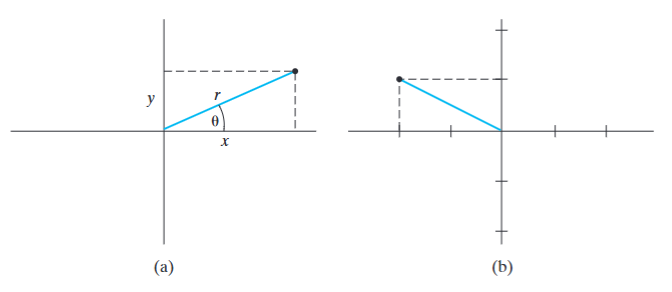
\includegraphics[width=0.8\textwidth]{1.3}
    \caption{（a）复数$z\ =\ x\ +\ iy$（b）复数$-2\ +\ i$图}
    \label{pic1.3}
\end{figure}
如果$z$是实数，则其虚部为零。因此当且仅当$z\ =\ z^*$时$z$为实数。取复共轭两次则重新得到$z$，$(z^*)^*\ =\ z$。将$z$与其复共轭相乘，利用$i^2\ =\ -1$，我们有
\begin{gather}
    zz^*\ =\ (x\ +\ iy)(x\ -\ iy)\ =\ x^2\ +\ iyx\ -\ iyx\ -\ i^2y^2 \notag \\
    \boxed{zz^*\ =\ x^2\ +\ y^2\ =\ r^2\ =\ \left|z\right|^2}
\end{gather}

对于两个复数$z_1\ =\ r_1e*{i\theta_1}$和$z_2\ =\ r_2e*{i\theta_2}$的乘积和商，有两个维度在这个范围内的就是
\begin{equation}
    z_1z_2\ =\ r_1r_2e^{i(\theta_1\ +\ \theta_2)},\ \frac{z_1}{z_2}\ =\ \frac{r_1}{r_2}e^{i(\theta_1\ -\ \theta_2)}
    \label{eq1.31}
\end{equation}

无论是从复共轭的定义还是从\eqref{eq1.31}，都易证明
\begin{equation}
    \boxed{(z_1z_2)^*\ =\ z_1^*z_2^*}
\end{equation}
相似的，
\begin{equation}
    \boxed{(z_1/z_2)^*\ =\ z_1^*/z_2^*,\quad(z_1\ +\ z_2)^*\ =\ z_1^*\ +\ z_2^*,\quad(z_1\ -\ z_2)^*\ =\ z_1^*\ -\ z_2^*}
\end{equation}
对于积与商的绝对值，从\eqref{eq1.31}可得
\begin{equation}
    \left|z_1z_2\right|\ =\ \left|z_1\right|\left|z_2\right|,\quad\left|\frac{z_1}{z_2}\right|\ =\ \frac{\left|z_1\right|}{\left|z_2\right|}
\end{equation}
因此，若$\psi$是一个复波函数，我们共有
\begin{equation}
    \left|\psi^2\right|\ =\ \left|\psi\right|^2\ =\ \psi^*\psi
\end{equation}

我们现在推导出1的$n$次方根的公式。我们可选取数字1的相位为$0$或$2\pi$或$4\pi$，以此类推。因此$1\ =\ e^{i2\pi k}$，其中$k$是任意整数，零，负的或正的都可以。现在考虑数$\omega\ \equiv\ e^{i2\pi k/n}$，$n$为一个正整数。使用\eqref{eq1.31}$n$次，我们看到$\omega^n\ =\ e^{i2\pi k}\ =\ 1$。因此$\omega$是$n$次的单位根。共有$n$个不同的复$n$次的单位根，再取$n$个连续的整数$k$值给出所有的单位根：
\begin{equation}
    \omega\ =\ e^{i2\pi k/n},\quad k\ =\ 0,1,2,……,n\ -\ 1
    \label{eq1.36}
\end{equation}
用\eqref{eq1.36}外其他的$k$值都将会给出一个相位，其总会与使用\eqref{eq1.36}中某个$k$值所得的相位差$2\pi$的整数倍。对于\eqref{eq1.36}中$n\ =\ 2$的情况，我们可得到两个1的平方根；对于$n\ =\ 3$，得到三个1的立方根；以此类推。
\end{flushleft}
\section{单位}
\begin{flushleft}
    \setlength{\parindent}{2em}
本书使用$SI$单位。在国际单位制（$SI$）中，长度、质量和时间的单位分别为米（m）、千克（kg）、和秒（s）。力以牛顿（N）衡量，能量以焦耳（J）衡量。两个真空中间隔$r$的电荷$Q_1$和$Q_2$之间力的大小的库伦定律由$SI$单位写作
\begin{equation}
    \boxed{F\ =\ \frac{Q_1Q_2}{4\pi \varepsilon_0r^2}}
\end{equation}
其中电荷$Q_1$和$Q_2$的单位为库伦（C），$\varepsilon_0$是常数（称为\textbf{真空介电常数}或\textbf{电常数}），其值为$8.854\ \times\ 10^{-12}\ C^2N^{-1}m^{-2}$（见物理常数准确值附录）。
\end{flushleft}
\section{微积分}
\begin{flushleft}
    \setlength{\parindent}{2em}
积分在量子化学中用得极多，下面的几个公式应当记住。其中$c$、$n$、$b$是常数，$f$和$g$是$x$的函数。
\begin{gather*}
    \boxed{\frac{\mathrm{d}c}{\mathrm{d}x}\ =\ 0,\quad\frac{\mathrm{d}(cf)}{\mathrm{d}x}\ =\ c\frac{\mathrm{d}f}{\mathrm{d}x},\quad\frac{\mathrm{d}x^n}{\mathrm{d}x}\ =\ nx^{n\ -\ 1},\quad\frac{\mathrm{d}e^{cx}}{\mathrm{d}x}\ =\ ce^{cx}} \\
    \boxed{\frac{\mathrm{d}(\sin cx)}{\mathrm{d}x}\ =\ c\cos cx,\quad\frac{\mathrm{d}(\cos cx)}{\mathrm{d}x}\ =\ -c\sin cx,\quad\frac{\mathrm{d}\ln cx}{\mathrm{d}x}\ =\ \frac{1}{x}} \\
    \boxed{\frac{\mathrm{d}(f\ +\ g)}{\mathrm{d}x}\ =\ \frac{\mathrm{d}f}{\mathrm{d}x}\ +\ \frac{\mathrm{d}g}{\mathrm{d}x},\quad\frac{\mathrm{d}(fg)}{\mathrm{d}x}\ =\ f\frac{\mathrm{d}g}{\mathrm{d}x}\ +\ g\frac{\mathrm{d}f}{\mathrm{d}x}} \\
    \boxed{\frac{\mathrm{d}(f/g)}{\mathrm{d}x}\ =\ \frac{\mathrm{d}(fg^{-1})}{\mathrm{d}x}\ =\ -fg^{-2}\frac{\mathrm{d}g}{\mathrm{d}x}\ +\ g^{-1}\frac{\mathrm{d}f}{\mathrm{d}x}} \\
    \boxed{\frac{\mathrm{d}}{\mathrm{d}x}f(g(x))\ =\frac{\mathrm{d}f}{\mathrm{d}g}\frac{\mathrm{d}g}{\mathrm{d}x}}
\end{gather*}

最后一条式子的一个例子为$\mathrm{d}[\sin(cx^2)]\ =\ 2cx\cos(cx^2)$。此处$g(x)\ =\ cx^2$而$f\ =\ \sin$。
\begin{gather*}
    \boxed{\int cf(x)\mathrm{d}x\ =\ c\int f(x)\mathrm{d}x,\quad\int [f(x)\ +\ g(x)]\mathrm{d}x\ =\ \int f(x)\mathrm{d}x\ +\ \int g(x)\mathrm{d}x} \\
    \boxed{\int \mathrm{d}x\ =\ x,\quad\int x^n\mathrm{d}x\ =\ \frac{x^{n\ +\ 1}}{n\ +\ 1}\text{当}n\ \neq\ -1\text{时},\quad\int \frac{1}{x}\mathrm{d}x\ =\ \ln x} \\
    \boxed{\int e^{cx}\mathrm{d}x\ =\ \frac{e^{cx}}{c},\quad\int \sin cx\mathrm{d}x\ =\ -\frac{\cos cx}{c},\quad\int \cos cx\mathrm{d}x\ =\ \frac{\sin cx}{c}} \\
    \boxed{\int_b^c f(x)\mathrm{d}x\ =\ g(c)\ -\ g(b)\quad\text{其中}\frac{\mathrm{d}g}{\mathrm{d}x}\ =\ f(x)}
\end{gather*}
\end{flushleft}
\section*{总结}
\begin{flushleft}
一个量子力学系统的状态通过一个状态函数或波函数$\bm{\Psi}$来描述，其是系统中粒子坐标和时间的函数。状态函数根据含时薛定谔方程随时间改变而改变，对于单粒子单维度系统而言为公式\eqref{eq1.13}。对于这样一个系统，$\left|\bm{\Psi(x,t)}\right|^2\mathrm{d}x$给出$t$时刻一次对粒子位置的测量\pdfcomment{无损测量，概率来自于不确定原理这一量子力学本质}在$x$与$x\ +\ \mathrm{d}x$之间发现粒子的概率。状态函数根据公式$\int_{-\infty}^{\infty}\left|\bm{\Psi}\right|^2\mathrm{d}x\ =\ 1$被归一化。若系统的势能不随时间$t$改变，则系统能以大量的恒定能量定态中某一个存在。对于一个单粒子单维度系统的定态，$\bm{\Psi}(x,t)\ =\ e^{-iEt/\hbar}\psi(x)$，其中与时间无关的波函数$\psi(x)$是定态薛定谔方程\eqref{eq1.19}的一个解。
\end{flushleft}
\section*{习题}
见原书

\chapter{势箱中的粒子}
\begin{flushleft}
通过解定态薛定谔方程\eqref{eq1.19}，可以获得单粒子单维度系统的定态波函数和能级。在本章中，我们将求解一个非常简单的系统的定态薛定谔方程，一维势箱中的粒子（2.2小节）。因为薛定谔方程是微分方程，我们先来讨论薛定谔方程。
\end{flushleft}
\section{微分方程}
\begin{flushleft}
    \setlength{\parindent}{2em}
本小节只考虑\textbf{常微分方程}，其只有一个独立变量。[\textbf{偏微分方程}有超过一个独立变量。含时薛定谔方程\eqref{eq1.16}便是一个例子，其中$t$和$x$是独立变量。]常微分方程是一个独立变量$x$，一个相关变量$y(x)$，和$y$的一阶、二阶……$n$阶导数（$y'$，$y''$，……，$y^{(n)}$）之间的关系。一个例子是
\begin{equation}
    y'''\ +\ 2x(y')^2\ +\ y^2\sin x\ =\ 3e^x
    \label{eq2.1}
\end{equation}
微分方程的\textbf{阶数}是方程中最高阶导数的阶数。因而\eqref{eq2.1}是三阶方程。

微分方程一种特殊形式为\textbf{线性微分方程}，其形式为
\begin{equation}
    A_n(x)y^{(n)}\ +\ A_{n-1}(x)y^{(n-1)}\ +\ \dots\ +\ A_1(x)y'\ +\ A_0(x)y\ =\ g(x)
    \label{eq2.2}
\end{equation}
其中所有$A$类和$g$（有些可能为零）仅是$x$的函数。在$n$阶线性微分方程\eqref{eq2.2}中，$y$和其导数都是一次幂。无法写成\eqref{eq2.2}形式的微分方程是\textbf{非线性}的。若\eqref{eq2.2}中$g(x)\ =\ 0$，则该线性微分方程是\textbf{齐次}的；否则是\textbf{非齐次}的。一维薛定谔方程\eqref{eq1.19}是线性齐次二阶微分方程。

通过除以$y''$的系数，我们可以把每个线性齐次二阶微分方程写成
\begin{equation}
    y''\ +\ P(x)y'\ +\ Q(x)y\ =\ 0
    \label{eq2.3}
\end{equation}
的形式。考虑两个独立且均满足\eqref{eq2.3}的函数$y_1$和$y_2$。独立的意思是$y_2$不是$y_1$的简单倍数。则线性齐次微分方程\eqref{eq2.3}的通解为
\begin{equation}
    y\ =\ c_1y_1\ +\ c_2y_2
    \label{eq2.4}
\end{equation}
其中$c_1$和$c_2$是任意常数。这可以通过将\eqref{eq2.4}代入\eqref{eq2.3}的左侧证明：
\begin{align}
    &c_1y_1''\ +\ c_2y_2''\ +\ P(x)c_1y_1'\ +\ P(x)c_2y_2'\ +\ Q(x)c_1y_1\ +\ Q(x)c_2y_2 \notag \\
    &=\ c_1[y_1''\ +\ P(x)y_1'\ +\ Q(x)y_1]\ +\  c_2[y_2''\ +\ P(x)y_2'\ +\ Q(x)y_2] \notag \\
    &=\ c_1\ \cdot\ 0\ +\ c_2\ \cdot\ =\ 0
\end{align}
其中使用到了$y_1$和$y_2$符合\eqref{eq2.3}的条件。

$n$阶微分方程的通解一般有$n$个任意常数。为了确定这些常数，我们需要\textbf{边界条件}，即在一个点或多个点上确定$y$或其各阶导数的条件。比如，如果$y$是系在两个点之间振动弦的位移，我们知道某些点上$y$必须为0。

一个重要的特例是\textbf{常系数}线性齐次二阶微分方程：
\begin{equation}
    y''\ +\ py'\ +\ qy\ =\ 0
    \label{eq2.6}
\end{equation}
其中$p$和$q$是常数。为了求解\eqref{eq2.6}，我们尝试$y\ =\ e^{sx}$形式的解。我们在找一个函数，其导数乘以常数可以消去原本的函数。指数函数在求导时会保持其原有形式，是一个正确的选择。代入\eqref{eq2.6}得到
\begin{gather}
    s^2e^{sx}\ +\ pse^{sx}\ +\ qe^{sx}\ =\ 0 \notag \\
    \boxed{s^2\ +\ ps\ +\ q\ =\ 0}
    \label{eq2.7}
\end{gather}
\eqref{eq2.7}被称为\textbf{辅助方程}。它是一个一元二次方程，当根$s_1$和$s_2$不相等时有两个根，给出两个\eqref{eq2.6}的独立解。因而，\eqref{2.6}的通解为
\begin{equation}
    \boxed{y\ =\ c_1e^{s_1x}\ +\ c_2e^{s_21x}}
    \label{eq2.8}
\end{equation}
比如，对于$y''\ +\ 6y'\ -\ 7y\ =\ 0$，辅助方程为$s^2\ +\ 6s\ -\ 7\ =\ 0$。该一元二次方程给出$s_1\ =\ 1$，$s_2\ =\ -7$，所以通解为$c_1e^x\ +\ c_2e^{-7x}$。
\end{flushleft}
\section{一维势箱中的粒子}
\begin{flushleft}
    \setlength{\parindent}{2em}
这一小节求解一维势箱中一个粒子的定态薛定谔方程。这里我们指一个粒子其势函数满足，在$x$轴上一个长度$l$的线段上为零，其余所有地方为无限大。这样的系统在物理上看起来是不现实的，但这个模型可以较成功地应用于确定的共轭分子；见习题2.17。我们将原点设置在这一线段的左端（图\eqref{pic2.1}）。
\begin{figure}[hbtp]
    \centering
    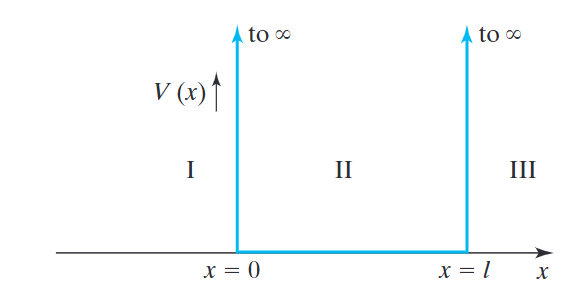
\includegraphics[width=0.8\textwidth]{2.1}
    \caption{一维势箱中粒子的势函数$V(x)$}
    \label{pic2.1}
\end{figure}

我们要考虑三个区域。在区域I和区域III中，势函数$V$等于无限大，定态薛定谔方程\eqref{eq1.19}为一个正整数
\begin{equation*}
    -\frac{\hbar^2}{2m}\frac{\mathrm{d}^\psi}{\mathrm{d}x^2}\ =\ (E\ -\ \infty)\psi
\end{equation*}
相较于$\infty$，$E$可忽略，我们可以得到
\begin{equation*}
    \frac{\mathrm{d}^2}\psi{\mathrm{d}x^2}\ =\ \infty\psi,\quad\psi\ =\ \frac{1}{\infty}\frac{\mathrm{d}^2\psi}{\mathrm{d}x^2}
\end{equation*}
因而我们得到$\psi$在盒外为零：
\begin{equation}
    \psi_I\ =\ 0,\quad\psi_{III}\ =\ 0
\end{equation}

对于区域II，$x$位于0与$l$之间，势函数$V$为零，薛定谔方程\eqref{eq1.19}变为
\begin{equation}
    \frac{\mathrm{d}^2\psi_{II}}{\mathrm{d}x^2}\ +\ \frac{2m}{\hbar}E\psi_{II}\ =\ 0
    \label{eq2.10}
\end{equation}
其中$m$是粒子的质量，$E$为其能量。我们认出\eqref{eq2.10}是常系数线性齐次二阶微分方程。辅助方程\eqref{eq2.7}给出
\begin{gather}
    s^2\ +\ 2mE\hbar^{-2}\ =\ 0 \notag \\
    s\ =\ \pm(-2mE)^{1/2}\hbar^{-1} \label{eq2.11}\\
    s\ =\ \pm i(2mE)^{1/2}\hbar^{-1} \label{eq2.12}
\end{gather}
其中$i\ \equiv\ \sqrt{-1}$。利用\eqref{eq2.8}，我们共有
\begin{equation}
    \psi_{II}\ =\ c_1e^{i(2mE)^{1/2}x/\hbar}\ +\ c_2e^{-i(2mE)^{1/2}x/\hbar}
    \label{eq2.13}
\end{equation}
暂时的，我们令
\begin{gather*}
    \theta\ \equiv\ (2mE)^{1/2}x/\hbar
    \psi_{II}\ =\ c_1e^{i\theta}\ +\ c_2e^{-i\theta}
\end{gather*}
我们有$e^{i\theta}\ =\ \cos\theta\ +\ i\sin\theta$[公式\eqref{eq1.28}]，$e^{-i\theta}\ =\ \cos(-\theta)\ +\ i\sin(-\theta)\ =\ \cos\theta\ -\ i\sin\theta$，因为
\begin{equation}
    \boxed{\cos(-\theta)\ =\ \cos\theta,\sin(-\theta)\ =\ -\sin\theta}
\end{equation}
因此，
\begin{align*}
    \psi_{II}\ &=\ c_1\cos\theta\ +\ ic_1\sin\theta\ +\ c_2\cos\theta\ -\ ic_2\sin\theta \\
    &=\ (c_1\ +\ c_2)\cos\theta\ +\ (ic_1\ -\ ic_2)\sin\theta \\
    &=\ A\sin\theta\ +\ B\sin\theta
\end{align*}
其中$A$和$B$是新的任意常数。因而，
\begin{equation}
    \psi_{II}\ =\ A\cos[\hbar^{-1}(2mE)^{1/2}x]\ +\ B\sin[\hbar^{-1}(2mE)^{1/2}x]
    \label{eq2.15}
\end{equation}

现在我们通过施加边界条件来获得$A$和$B$。假定波函数是连续的似乎很合理；这是指，它的值不会突跃（见图\eqref{pic3.4}）。若$\psi$在$x\ =\ 0$处是连续的，那么$\psi_I$和$\psi_{II}$都必须在$x\ =\ 0$处接近同一值：
\begin{align*}
    \lim_{x\to 0}\psi_I\ &=\ \lim_{x\to 0}\psi_{II} \\
    0\ &=\ \lim_{x\to 0}\{A\cos[\hbar^{-1}(2mE)^{1/2}x]\ +\ B\sin[\hbar^{-1}(2mE)^{1/2}x]\} \\
    0\ =\ A
\end{align*}
因为
\begin{equation}
    \boxed{\sin 0\ =\ 0,\ \cos 0\ =\ 1}
\end{equation}
由于$A\ =\ 0$，公式\eqref{eq2.15}变为
\begin{equation}
    \psi_{II}\ =\ B\sin[(2\pi/h)(2mE)^{1/2}x]
    \label{eq2.17}
\end{equation}
在$x\ =\ l$处应用该连续性条件，我们得到
\begin{equation}
    B\sin[(2\pi/h)(2mE)^{1/2}l]\ =\ 0
\end{equation}
$B$不能为零，因为这会使波函数到处都是零——我们将得到一个空势箱。因此，
\begin{equation*}
    \sin[(2\pi/h)(2mE)^{1/2}l]\ =\ 0
\end{equation*}
正弦函数的零值出现在$0$，$\pm\pi$，$\pm 2\pi$，$\pm 3\pi$，……，$\pm n\pi$。因此，
\begin{equation}
    (2\pi/h)(2mE)^{1/2}l\ =\ \pm n\pi
    \label{eq2.19}
\end{equation}

$n\ =\ 0$是一个特例。\eqref{eq2.19}中，$n\ =\ 0$对应着能量$E\ =\ 0$。对于$E\ =\ 0$，辅助方程的根\eqref{eq2.12}相等，则\eqref{eq2.13}不再是薛定谔方程完备解的表达式。为了得到完备解，我们回到\eqref{eq2.10}，对于$E\ =\ 0$可写为$\frac{\mathrm{d}^2\psi_{II}}{\mathrm{d}x^2}\ =\ 0$。积分得到$\frac{\mathrm{d}\psi_{II}}{\mathrm{d}x}\ =\ c$，$\psi_{II}\ =\ cx\ +\ d$，其中$c$和$d$是常数。边界条件$x\ =\ 0$处$\psi_{II}\ =\ 0$给出$d\ =\ 0$，而条件$x\ =\ l$处$\psi_{II}\ =\ 0$给出$c\ =\ 0$。因此，$E\ =\ 0$时$\psi_{II}\ =\ 0$，故$E\ =\ 0$不是允许的能量值。因此$n\ =\ 0$不被允许。

求解$E$，我们有
\begin{equation}
    \boxed{E\ =\ \frac{n^2h^2}{8ml^2}\quad n\ =\ 1,2,3,\dots}
    \label{eq2.20}
\end{equation}

只有\eqref{eq2.20}的能量值允许$\psi$满足$x\ =\ l$处连续性的边界条件。边界条件的应用使我们得到能量值量子化的结论（图\eqref{pic2.2}）。这与势箱中粒子可以具有任意非负能量的经典结论产生鲜明矛盾。注意到粒子的能量存在大于零的最小值。能量最低的状态被称为\textbf{基态}。能量高于基态基态能量的状态为\textbf{激发态}。（在经典力学中，势箱内一个粒子的最低可能能量为零。该经典粒子在势箱中静止不动，动能和势能均为零。）
\begin{figure}[hbtp]
    \centering
    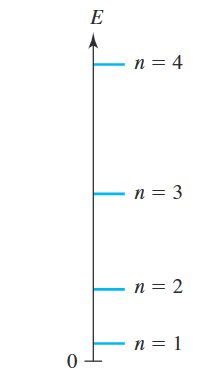
\includegraphics[width=0.8\textwidth]{2.2}
    \caption{一维势箱中粒子最低的4个能级}
    \label{pic2.2}
\end{figure}

\begin{examplebox}
    \setlength{\parindent}{2em}
\noindent 质量为$2.00\ \times\ 10^{-26}$的粒子位于长度为$4.00\ \text{nm}$的一维势箱中。求出当该粒子从能级$n\ =\ 3$到$n\ =\ 2$时，发射出光子的频率和波长。

根据能量守恒，发射光子的能量$h\nu$等于两个定态之间的能量差[\eqref{eq1.4}；此外见小节9.9]：
\begin{gather*}
    h\nu\ =\ E_{upper}\ -\ E_{lower}\ =\ \frac{n_u^2h^2}{8ml^2}\ -\ \frac{n_l^2h^2}{8ml^2} \\
    \nu\ =\ \frac{(n_u^2\ -\ n_l^2)h}{8ml^2}\ =\ \frac{(3^2\ -\ 2^2)(6.626\ \times\ 10^{-34}\ \text{J}\cdot\text{s})}{8(2.00\ \times\ 10^{-29}\ \text{kg})(4.00\ \times\ 10^{-9}\ \text{m})^2}\ =\ 1.29\ \times\ 10^{12}\ \text{s}^{-1}
\end{gather*}
其中$u$和$l$代表高能级与低能级。使用$\lambda\nu\ =\ c$给出$\lambda\ =\ 2.32\ \times\ 10^{-4}\ \text{m}$。（一个学生常犯的错误是，将$h\nu$等于一个能级的能量而不是能级间的\textit{能量差}。）

\noindent \textcolor{blue}{\large 练习}\ 对于在一个确定的一维势箱中的电子，最长的跃迁波长在$400\ \text{nm}$。求出势箱长度。（答案：$0.603\ \text{nm}$。）
\end{examplebox}

将\eqref{eq2.19}代入\eqref{eq2.17}给出波函数
\begin{equation}
    \psi_{II}\ =\ B\sin(\frac{n\pi x}{l}),\quad n\ =\ 1,2,3,\dots
    \label{eq2.21}
\end{equation}
在$n\pi$前面加上负号不会给出新的独立解。因为$\sin(-\theta)\ =\ -\sin\theta$，我们可以简单地得到常数$-1$，来乘以带正号的解。

公式\eqref{eq2.21}中的$B$仍是任意的。为了确定其值，我们使用归一化要求，公式\eqref{eq1.24}和\eqref{eq1.22}：
\begin{gather}
    \int_{-\infty}^{\infty}\left|\Psi\right|^2\mathrm{d}x\ =\ \int_{-\infty}^{\infty}\left|\psi\right|^2\mathrm{d}x\ =\ 1 \notag \\
    \int_{-\infty}^{\infty}\left|\psi_I\right|^2\mathrm{d}x\ +\ \int_{-\infty}^{\infty}\left|\psi_{II}\right|^2\mathrm{d}x\ +\ \int_{-\infty}^{\infty}\left|\psi_{III}\right|^2\mathrm{d}x\ =\ 1 \notag \\
    \left|B\right|^2\int_0^l\sin^2(\frac{n\pi x}{l})\mathrm{d}x\ =\ 1\ =\ \left|B\right|^2\frac{l}{2}
    \label{eq2.22}
\end{gather}
其中积分通过附录中的公式\eqref{eqA.2}计算。我们有
\begin{equation*}
    \left|B\right|\ =\ (2/l)^{1/2}
\end{equation*}

注意到只求得$B$的绝对值。$B$可以为$(2/l)^{1/2}$和$-(2/l)^{1/2}$。此外，$B$不必为实数。我们可以用任何绝对值为$(2/l)^{1/2}$的复数。我们能说的是$B\ =\ (2/l)^{1/2}e^{i\alpha}$，其中$\alpha$是$B$的相位且可以是$0$到$2\pi$的任意值（1.7小节）。选择相位为零，我们将其写作势箱中粒子的定态波函数
\begin{equation}
    \boxed{\psi_{II}\ =\ (\frac{2}{l})^{1/2}\sin(\frac{n\pi x}{l}),\quad n\ =\ 1,2,3,\dots}
    \label{eq2.23}
\end{equation}

波函数和概率密度的图像如图\eqref{pic2.3}和\eqref{pic2.4}所示。
\begin{figure}[hbtp]
    \centering
    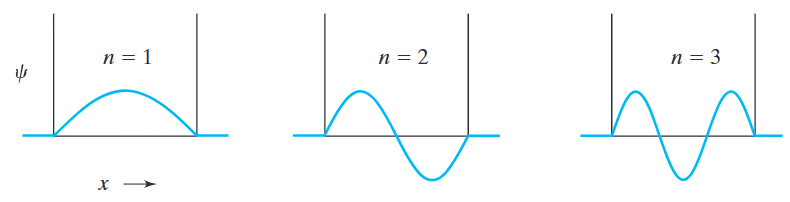
\includegraphics[width=0.8\textwidth]{2.3}
    \caption{势箱中粒子三个最低能量状态$\psi$图像}
    \label{pic2.3}
\end{figure}
\begin{figure}[hbtp]
    \centering
    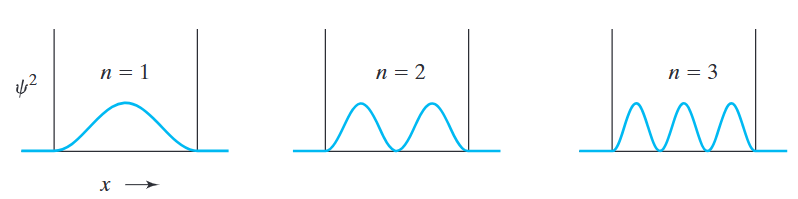
\includegraphics[width=0.8\textwidth]{2.4}
    \caption{势箱中粒子三个最低能量状态$\left|\psi\right|^2$图像}
    \label{pic2.4}
\end{figure}

能量\eqref{eq2.20}和波函数\eqref{eq2.23}中数字$n$被称为\textbf{量子数}。每个不同的量子数$n$给出一个不同的波函数和不同的状态。

波函数在一些确定的点上为零；这些点被称为\textbf{节点}。量子数$n$每增加1，$\psi$将多一个节点。$\psi$和$\left|\psi\right|^2$中节点的存在也许让人吃惊。对于$n\ =\ 2$，图\eqref{pic2.4}表明在盒子中间$x\ =\ l/2$处找到粒子的概率为零。该粒子怎么能从势箱的一侧去到另一侧而在任何时候都不在中间被发现？这个明显的悖论来自于用日常生活中宏观粒子运动的经验去尝试理解微观粒子的运动。然而，正如第一章注意到的那样，电子和其他微观“粒子”不能被完全且正确地从由宏观世界取得的经典物理概念来描述。

图\eqref{pic2.4}表明在势箱的不同地方找到粒子的概率与经典结果相当不同。经典力学中，箱中具有固定能量的粒子在两壁之间来回弹性反弹，以恒定速度运动。因此它等可能的在箱中各点被发现。量子力学上，我们发现最低能级下在箱中央为概率的极大值。随着能级升高，节点变多，概率的极大值和极小值逐渐接近，最终沿着势箱长度概率的变化变得无法分辨。对于非常高的量子数，体系趋近于均匀概率密度的经典结果。

在量子数趋于极大时量子力学趋近于经典力学的结论被称为\textit{Bohr对应原理}。因为牛顿力学控制宏观物体（运动速度远小于光速），我们希望非相对论量子力学对宏观物体给出与经典力学相同的结论。因为Planck常数数值极小，宏观物体能量的量子化难以观察。因为粒子的质量和势箱长度的平方出现在公式\eqref{eq2.20}的分母中，一个具有宏观运动能量，位于宏观势箱内的宏观物体将会有很大的$n$值\pdfcomment{这个推n很大的说法有点古怪}，因此，根据对应原理，将会表现出经典行为。

我们现在有一整组波函数，每一个都对应于一个不同的能量，以正整数量子数$n$为特征。令角标$i$标志以$n_i$为量子数的特定波函数：
\begin{gather*}
    \psi_i\ =\ (\frac{2}{l})^{1/2}\sin(\frac{n_i\pi x}{l}),\ 0 \leq\ x\ \leq\ l \\
    \psi_i\ =\ 0\ \text{别处}
\end{gather*}
因为波函数是归一化的，我们有
\begin{equation}
    \int_{-\infty}^{\infty}\psi_i^*\psi_j\mathrm{d}x\ =\ 1,\ \text{当}i\ =\ j 
    \label{eq2.24}
\end{equation}
我们现在求当使用对应于\textit{不同}能级的波函数积分的值：
\begin{equation*}
    \int_{-\infty}^{\infty}\psi_i^*\psi_j\mathrm{d}x\ =\ \int_0^l(\frac{2}{l})^{1/2}\sin(\frac{n_i\pi x}{l})(\frac{2}{l})^{1/2}\sin(\frac{n_j\pi x}{l})\mathrm{d}x,\quad n_i\ \neq\ n_j
\end{equation*}
利用附录中公式\eqref{eqA.5}给出
\begin{equation}
    \int_{-\infty}^{\infty}\psi_i^*\psi_j\mathrm{d}x\ =\ \frac{2}{l}[\frac{\sin[(n_i\ -\ n_j)\pi]}{2(n_i\ -\ n_j)\pi/l}\ -\ \frac{\sin[(n_i\ +\ n_j)\pi]}{2(n_i\ +\ n_j)\pi/l}]\ =\ 0
    \label{eq2.25}
\end{equation}
因为对于整数$m$，$\sin m\pi\ =\ 0$。我们因此有
\begin{equation}
    \int_{-\infty}^{\infty}\psi_i^*\psi_j\mathrm{d}x\ =\ 0,\quad i\ \neq\ j
    \label{eq2.26}
\end{equation}
当\eqref{eq2.26}成立时，函数$\psi_i$和$\psi_j$彼此被称为\textbf{正交}。我们将\eqref{eq2.24}和\eqref{eq2.26}结合，写作
\begin{equation}
    \int_{-\infty}^{\infty}\psi_i^*\psi_j\mathrm{d}x\ =\ \delta_{ij}
    \label{eq2.27}
\end{equation}
记号$\delta_{ij}$被称为\textbf{Kronecker符号}（以数学家名字命名）。它在两个索引$i$和$j$相同时等于1，不相同时等于0：
\begin{equation}
    \boxed{\delta_{ij} \equiv
    \begin{cases} 
    0 & ,i \neq j \\
    1 & ,i = j 
    \end{cases}}
\end{equation}
\eqref{eq2.27}表示的波函数性质称为\textbf{正交性}。我们仅证明了势箱中粒子波函数的正交性。我们将在7.2小节更普适地证明它。

你可能会对\eqref{eq2.26}感到疑惑，想知道为什么我们要将一种状态的波函数乘以另一种不同状态的波函数。后面我们会看到（例如7.3小节），使用含有囊括系统所有波函数的和的等式一般很有帮助，而这样的等式会带来像\eqref{eq2.26}的积分。

一种更严谨地看待无限势垒势箱中粒子的方式为，先将其看作粒子处于势垒处势能仅为有限的突跃，随后将$V$的突跃趋于极限，变得无穷大。当极限取到时，结果将与\eqref{eq2.20}和\eqref{eq2.23}相同（见习题2.22）。

我们只考虑了一维势箱中粒子的定态。对于该系统非定态的例子，见7.8小节靠近结尾的案例。

一些势箱中粒子的在线计算机模拟可以在\url{www.chem.uci.edu/undergraduate/applets/dwell/dwell.htm}（展示当一个高度与宽度可变势垒被引入势箱中间时波函数受到的影响）；\url{web.williams.edu/wp-etc/chemistry/dbingemann/Chem153/particle.htm}（通过画出随着能量、势箱长度变化薛定谔方程的解来展示量子化）；和\url{falstad.com/qm1d/}（展示定态和随时演化状态；见习题7.47）找到。
\end{flushleft}
\section{一维自由粒子}
\begin{flushleft}
    \setlength{\parindent}{2em}
讲自由粒子，意味着一个无论怎样都不受力的粒子。对于一个自由粒子，\eqref{eq1.12}的积分表明无论$x$的值是多少，势能恒定不变。因为势能零级的选择是任意的，我们设定$V(x)\ =\ 0$。薛定谔方程\eqref{eq1.19}变为
\begin{equation}
    \frac{\mathrm{d}^2\psi}{\mathrm{d}x^2}\ +\ \frac{2m}{\hbar^2}E\psi\ =\ 0
    \label{eq2.29}
\end{equation}
公式\eqref{eq2.29}和公式\eqref{eq2.10}（除了边界条件）。因此，\eqref{eq2.29}的通解为\eqref{eq2.13}：
\begin{equation}
    \psi\ =\ c_1e^{i(2mE)^{1/2}x/\hbar}\ +\ c_2e^{-i(2mE)^{1/2}x/\hbar}
    \label{eq2.30}
\end{equation}

我们应该加上什么边界条件？假定（因为$\psi^*\psi\mathrm{d}x$表示概率）当$x$趋向$\pm\infty$时$\psi$保存有限看起来很合理。若能量$E$小于零，则违背这条边界条件，因为$E\ <\ 0$时我们有
\begin{equation*}
    i(2mE)^{1/2}\ =\ i(-2m\left|E\right|)^{1/2}\ =\ i\cdot i(2mE)^{1/2}\ =\ -(2mE)^{1/2}
\end{equation*}
因此\eqref{eq2.30}中第一项在$x$趋向于负无穷时会趋向无穷。相似的，若$E$为负数，\eqref{eq2.30}中第二项在$x$趋向于正无穷时会趋向无穷。因此边界条件要满足
\begin{equation}
    E\ \geq\ 0
\end{equation}
其波函数是振荡的，是一个正弦项和余弦项的线性组合[公式\eqref{eq2.25}]。对于自由粒子，其能量不是量子化的；所有非负能量都是允许的。因为我们设定$V\ =\ 0$，能量$E$在此案例中全部为动能。若我们尝试通过归一化计算任意常数$c_1$和$c_2$，我们会发现积分$\int_{-\infty}^{\infty}\psi^*(x)\psi(x)\mathrm{d}x$是无限的。换句话说，自由粒子波函数在通常意义下是不可归一化的。从物理学背景上这是预料到的，因为随着$x$趋近$\pm\infty$找到该自由粒子的概率趋于零是没有道理的。

自由粒子问题是不现实的情况，因为不可能真的有一个粒子不与宇宙中任何其他粒子存在作用。\pdfcomment{解释有点怪。应该说没有无限大的空间？}
\end{flushleft}
\section{方形势阱中的粒子}
\begin{flushleft}
    \setlength{\parindent}{2em}
现在考虑具有有限高势垒的一维势箱中的粒子（\eqref{pic2.5}（a））。在$x\ <\ 0$时势函数为$V\ =\ V_0$，$0\ \leq\ x\ \leq\ l$时$V\ =\ 0$，$x\ >\ l$时$V\ =\ V_0$。有两种情况要考虑，取决于粒子能量$E$大于还是小于$V_0$。
\begin{figure}[hbtp]
    \centering
    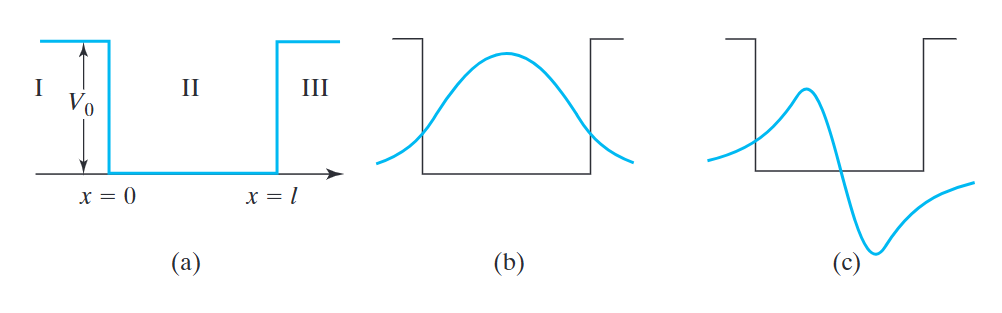
\includegraphics[width=0.8\textwidth]{2.5}
    \caption{（a）一维方势阱中一个粒子的势能（b）此势能下基态波函数（c）第一激发态波函数}
    \label{pic2.5}
\end{figure}

我们先考虑$E\ <\ V_0$的情况。区域I和III的薛定谔方程\eqref{eq1.19}为$\mathrm{d}^2\psi/\mathrm{d}x^2\ +\ (2m/\hbar^2)(E\ -\ V_0)\psi\ =\ 0$。这是常系数线性齐次微分方程，其辅助方程\eqref{eq2.7}为$s^2\ +\ (2m/\hbar^2)(E\ -\ V_0)\ =\ 0$，根为$s\ =\ \pm(2m/\hbar^2)^{1/2}(V_0\ -\ E)^{1/2}$。因此，
\begin{align*}
    \psi_I\ &=\ Cexp[(2m/\hbar^2)^{1/2}(V_0\ -\ E)^{1/2}x]\ +\ Dexp[-(2m/\hbar^2)^{1/2}(V_0\ -\ E)^{1/2}x] \\
    \psi_{III}\ &=\ Fexp[(2m/\hbar^2)^{1/2}(V_0\ -\ E)^{1/2}x]\ +\ Gexp[-(2m/\hbar^2)^{1/2}(V_0\ -\ E)^{1/2}x]
\end{align*}
其中$C$、$D$、$F$和$G$为常数。

正如小节2.3所说，我们必须防止$x\ \to\ -\infty$时$\psi_I$趋向无穷。因为我们假定$E\ <\ V_0$，$(V_0\ -\ E)^{1/2}$为正实数，所以为了让$x\ \to\ -\infty$时$\psi_I$有限，必须令$D\ =\ 0$。相似的，让$x\ \to\ +\infty$时$\psi_{III}$有限，必须令$F\ =\ 0$。因此，
\begin{equation*}
    \psi_I\ =\ Cexp[(2m/\hbar^2)^{1/2}(V_0\ -\ E)^{1/2}x],\quad\psi_{III}\ =\ Gexp[-(2m/\hbar^2)^{1/2}(V_0\ -\ E)^{1/2}x]
\end{equation*}

在区域II中，$V\ =\ 0$，薛定谔方程为\eqref{eq2.10}，其解为\eqref{eq2.15}：
\begin{equation}
    \psi_{II}\ =\ A\cos[(2m/\hbar^2)^{1/2}E^{1/2}x]\ +\ B\sin[(2m/\hbar^2)^{1/2}E^{1/2}x]
\end{equation}

为了完全解决问题，我们必须使用边界条件。正如无限高势垒势箱中的粒子一样，我们要求波函数在$x\ =\ 0$和$x\ =\ l$处连续；所以$\psi_I(0)\ =\ \psi_{II}(0)$，$\psi_{II}(0)\ =\ \psi_{III}(0)$。波函数有四个任意常数，所以需要更多的边界条件。正如要求$\psi$连续，我们应要求其导数$\mathrm{d}\psi/\mathrm{d}x$处处连续\pdfcomment{无限高一维势箱这俩边界条件也存在 ，只是给出的任意常数相同，多余了（？）}。为了证明这个要求正确，我们注意到如果$\mathrm{d}\psi/\mathrm{d}x$在某个点不连续改变，则它的导数（其瞬间变化率）$\mathrm{d}^2\psi/\mathrm{d}x^2$在该点为无穷。然而，对于方形势阱中的粒子，薛定谔方程$\mathrm{d}^2\psi/\mathrm{d}x^2\ =\ (2m/\hbar^2)(V\ -\ E)\psi$右侧不含有任何无限的项，所以$\mathrm{d}^2\psi/\mathrm{d}x^2$不能为无穷。[更严格的论证见D. Branson, \textit{Am. J. Phys.}, \textbf{47}, 1000 （1979）.]。因此，$x\ =\ 0$处$\mathrm{d}\psi_I/\mathrm{d}x\ =\ \mathrm{d}\psi_{II}/\mathrm{d}x$，$x\ =\ l$处$\mathrm{d}\psi_{II}/\mathrm{d}x\ =\ \mathrm{d}\psi_{III}/\mathrm{d}x$。

从$\psi_I(0)\ =\ \psi_{II}(0)$中我们得到$C\ =\ A$。从$\psi_I'(0)\ =\ \psi_{II}'(0)$中我们得到（习题2.21a）$B\ =\ (V_0\ -\ E)^{1/2}A/E^{1/2}$。从$\psi_{II}(0)\ =\ \psi_{III}(0)$中我们得到一条复杂的等式，使得$G$由$A$表示。常数$A$通过归一化求得。

对于$\psi_{II}'(0)\ =\ \psi_{III}'(0)$，将其除以$\psi_{II}(0)\ =\ \psi_{III}(0)$，将$B$表示为$A$的形式，我们得到如下的能级公式（习题2.21b）：
\begin{equation}
    (2E\ -\ V_0)\sin[(2mE)^{1/2}l/\hbar]\ =\ 2(V_0E\ -\ E^2)\cos[(2mE)^{1/2}l/\hbar]
    \label{eq2.33}
\end{equation}
[尽管$E\ =\ 0$满足\eqref{eq2.33}，其不是一个允许的能量值，因为它给出$\psi\ =\ 0$（习题2.30）。]定义无量纲常数$\varepsilon$和$b$为
\begin{equation}
    \varepsilon\ \equiv\ E/V_0\ \text{和}\ b\ \equiv\ (2mV_0)^{1/2}l/\hbar
\end{equation}
我们将\eqref{eq2.33}除以$V_0$得到
\begin{equation}
    (2\varepsilon\ -\ 1)\sin(b\varepsilon^{1/2})\ -\ 2(\varepsilon\ -\ \varepsilon^2)^{1/2}\cos(b\varepsilon^{1/2}\ =\ 0)
    \label{eq2.35}
\end{equation}
只有满足\eqref{eq2.33}的特定$E$值给出连续且导数连续的波函数，所以对于$E\ <\ V_0$能级是量子化的。为了找出允许的能级，我们可以将\eqref{eq2.35}的左侧对$\varepsilon$在$0\ <\ \varepsilon\ <\ 1$区间内的图作出来，然后找到曲线与水平轴的交点（同样见习题4.31c）。一个详细的研究（\textit{Merzbacher}，6.8小节）表明$E\ <\ V_0$时允许的能级的数量为$N$，$N$满足
\begin{equation}
    N\ -\ 1\ <\ b/\pi\ \leq\ N,\quad\text{其中}b\ \equiv\ (2mV_0)^{1/2}l/\hbar
    \label{eq2.36}
\end{equation}
例如，若$V_0\ =\ h^2/ml^2$，则$b/\pi\ =\ 2(2^{1/2})\ =\ 2.83$，$N\ =\ 3$。

图\eqref{pic2.5}展示最低两个能级的$\psi$。波函数在势箱中振荡，而在势箱外指数衰减。其表明能级每高一级节点数量增加1。

到现在我们只考虑了$E\ <\ V_0$的状态。对于$E\ >\ V_0$，$(V_0\ -\ E)^{1/2}$的值为虚数，与随着$x$趋近于$\pm\infty$衰减至零相反，$\psi_I$和$\psi_{III}$表现振荡（与自由粒子的$\psi$相似）。我们不再有理由去设置$\psi_I$中的$D$和$\psi_{III}$中的$F$为零，而有了这些额外的常数\pdfcomment{不是额外，而是少了无穷处的边界条件}去满足$\psi$和$\psi'$上的边界条件，我们发现不再需要限制$E$去获得性状良好的波函数。因此，所有大于$V_0$的能量都是允许的。

一个$x\ \to\ \pm\infty$时$\psi\ \to\ 0$的状态被称为\textbf{束缚态}。对于一个束缚态，仅在有限的空间区域里存在找到粒子的显著概率。对于一个\textbf{非束缚态（散射态，unbound state）}，$\psi$并不随$x\ \to\ \pm\infty$趋向零，因而不可归一化。对于方形势阱中的粒子，$E\ <\ V_0$的状态是束缚态，$E\ >\ V_0$的状态是非束缚态。对于无限高势垒势箱中的粒子，所有状态都是束缚态。对于自由粒子，所有状态都是非束缚态。

若想要势阱中粒子的在线模拟，可以去\url{www.falstad.com/qm1d}并在设置框中选择有限势阱。你可以改变势阱的宽度和深度，看看其对能级和波函数的影响。
\end{flushleft}
\section{隧穿}
\begin{flushleft}
    \setlength{\parindent}{2em}
对于方形势阱中的粒子（2.4小节），图\eqref{pic2.5}和$\psi_I$与$\psi_{III}$的公式表明对于总能量$E$小于势能$V\ =\ V_0$的束缚态，在区域I和III中没有地方找到粒子的概率为零。经典力学上，这种行为是不被允许的。经典公式$E\ =\ T\ +\ V$（$T$为动能）和$T\ \geq\ 0$意味着$E$在经典力学中不能小于$V$。

考虑一维势箱中的粒子，该势箱的势垒有限高\textit{且}有限厚（图\eqref{pic2.6}）。经典力学上，粒子无法逃出该势箱，除非其能量大于势垒$V_0$。然而，量子力学处理（此处省略）表明总能量小于$V_0$的粒子仍有有限的概率在势箱外被找到。
\begin{figure}[hbtp]
    \centering
    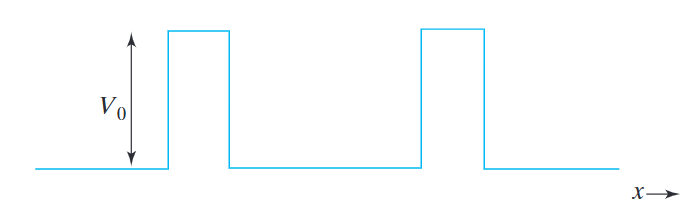
\includegraphics[width=0.8\textwidth]{2.6}
    \caption{势垒有限高有限厚的一维势箱中粒子的势能}
    \label{pic2.6}
\end{figure}

术语\textbf{隧穿}指粒子穿入经典上禁止的区域（如图\eqref{pic2.5}）或粒子穿过高于其能量势垒的过程。因为隧穿是一种量子效应，粒子的行为越不经典，隧穿出现的概率越大。因此，小质量粒子的隧穿更为普遍。（注意到质量$m$越大，2.4小节中函数$\psi_I$和$\psi_{III}$越快衰减到零。）电子很容易隧穿。氢原子和氢离子比其他更重的原子更容易隧穿。

$\alpha$粒子从一个放射性核发射的过程包含$\alpha$粒子隧穿通过由子核与$\alpha$粒子间短程吸引核力和库仑斥力产生的势垒。\ce{NH3}分子是三角锥形的。分子的翻转存在势垒，势能最大值出现在平面构型。氢原子可以隧穿通过该势垒，由此翻转分子\pdfcomment{这么说在接近绝对零度的时候氨分子也可以翻转？不必通过平面过渡态，无需外界提供活化能，仅靠氢原子的隧穿效应？}。在\ce{CH3CH3}中存在内部旋转的势垒，在氢原子处于重叠式时势能达到最大。氢原子可以隧穿通过该势垒，从一个交叉式位置到达另一个交叉式。电子的隧穿在氧化还原反应和电极过程中很重要。隧穿常对牵涉氢原子转移的化学反应的速率有很大贡献。见R. P. Bell, \textit{The Tunnel Effect in Chemistry}, Chapman \& Hall,1980。

$H$原子的隧穿在一些酶催化的反应中出现；见\textit{Quantum Tunnelling in Enzyme-Catalyzed Reactions}, R. Allemann and N. Scrutton (eds.), RSC Publishing, 2009。

扫描隧道显微镜于1981年发明，利用电子在一根金属丝的极细尖端与一导电固体表面之间的空间的隧穿，产生固体表面单个原子的图像。一个小电压被加在固体和金属线上，随着尖端在距离表面几埃的高度上移动越过表面，调整尖端高度使得电流恒定。尖端高度对位置作图给出表面的图像。
\end{flushleft}
\section*{总结}
\begin{flushleft}
    \setlength{\parindent}{2em}
线性、齐次、二阶、常系数微分方程$y''(x)\ +\ py'(x)\ +\ qy(x)\ =\ 0$的通解为$y\ =\ c_1e^{s_1x}\ +\ c_2e^{s_2x}$，其中$s_1$和$s_2$是辅助方程$s^2\ +\ ps\ +\ q\ =\ 0$的解。

对于一维势箱中的粒子（$0\ \leq\ x\ \leq\ l$时势能$V\ =\ 0$，其余地方$V\ =\ \infty$），定态波函数和能量为$0\ \leq\ x\ \leq\ l$时$\psi\ =\ (2/l)^{1/2}\sin(n\pi x/l)$，其他地方$\psi\ =\ 0$，$E\ =\ n^2h^2/8ml^2$，其中$n\ =\ 1,2,3,\dots$量子数$n$每增加1节点数（$\psi\ =\ 0$的地方）增加1。波函数是正交归一的[公式\eqref{eq2.27}]。

对于自由粒子（处处$V\ =\ 0$），所有非负能量都允许，且通常意义上波函数不可归一化。

有限高势垒的方形一维势阱中的粒子具有有限数量的束缚态[公式\eqref{eq2.36}]。束缚态波函数在势阱内是振荡的，在势阱外指数衰减至零。非束缚态的能量不是量子化的。

隧穿是一个粒子穿入经典上禁止的区域，或穿过高于粒子能量的势垒的过程。
\end{flushleft}
\section*{习题}
见原书

\chapter{算符}
\section{算符}
\begin{flushleft}
    \setlength{\parindent}{2em}
我们现在要以一种较之前更普适的方法发展量子力学。我们从写出以下形式的单粒子单维度定态薛定谔方程\eqref{eq1.19}开始
\begin{equation}
    [-\frac{\hbar^2}{2m}\frac{\mathrm{d}^2}{\mathrm{d}x^2}\ +\ V(x)]\psi(x)\ =\ E\psi(x)
    \label{eq3.1}
\end{equation}
\eqref{eq3.1}中中括号内的式子是一个\textit{算符}。公式\eqref{eq3.1}表明我们有了一个作用于波函数，重新给出波函数并乘以一个允许的能量值的算符。我们因此来讨论算符。

\textbf{算符}是将一个给定函数转变为另一个函数的规则。例如，$\hat{D}$是一个将函数对$x$微分的算符。我们在字母上方添加尖角符号$\hat{}$来表示算符。如果$f(x)$是可微的，则$\hat{D}$作用于$f(x)$的结果为$\hat{D}f(x)\ =\ f'(x)$。例如，$\hat{D}(x^2\ +\ 3e^{2x})\ =\ 2x\ +\ 6e^{2x}$。若$\hat{3}$为将函数乘以3，则$\hat{3}(x^2\ +\ 3e^x)\ =\ 3x^2\ +\ 9e^x$。若$\tan$是求函数正切值的算符，则将$\tan$用于函数$x^2\ +\ 1$给出$\tan(x^2\ +\ 1)$。若算符$\hat{A}$将函数$f(x)$转变为$g(x)$，则写作$\hat{A}f(x)\ =\ g(x)$。

我们定义两个算符$\hat{A}$和$\hat{B}$的\textbf{和}与\textbf{差}为
\begin{gather}
    \boxed{(\hat{A}\ +\ \hat{B})f(x)\ \equiv\ \hat{A}f(x)\ +\ \hat{B}f(x)} \label{eq3.2} \\
    (\hat{A}\ -\ \hat{B})f(x)\ \equiv\ \hat{A}f(x)\ -\ \hat{B}f(x) \notag
\end{gather}
比如，若$\hat{D}\ \equiv\ \mathrm{d}/\mathrm{d}x$，则
\begin{equation*}
    (\hat{D}\ +\ \hat{3})(x^3\ +\ 5)\ \equiv\ \hat{D}(x^3\ +\ 5)\ +\ \hat{3}(x^3\ +\ 5)\ =\ 3x^2\ +\ (3x^3\ -\ 15)\ =\ 3x^3\ +\ 3x^2\ -\ 15
\end{equation*}

一个算符可以不只包含一个变量。例如，算符$\partial^2/\partial x^2\ +\ \partial^2/\partial y^2$有以下作用
\begin{equation*}
    (\partial^2/\partial x^2\ +\ \partial^2/\partial y^2)g(x,y)\ =\ \partial^2g/\partial x^2\ +\ \partial^2g/\partial y^2
\end{equation*}

两个算符$\hat{A}$和$\hat{B}$的\textbf{乘积}被定义为
\begin{equation}
    \boxed{\hat{A}\hat{B}f(x)\ =\ \hat{A}[\hat{B}f(x)]}
    \label{eq3.3}
\end{equation}
换句话说，先用算符乘积右边的算符作用于$f(x)$，再用乘积左边的算符作用先前得到的函数。例如，$\hat{3}\hat{D}f(x)\ =\ \hat{3}[\hat{D}f(x)]\ =\ \hat{3}f'(x)\ =\ 3f'(x)$。

算符$\hat{A}\hat{B}$和$\hat{B}\hat{A}$未必具有相同的效果。比如考虑算符$\mathrm{d}/\mathrm{d}x$与$\hat{x}$（$\hat{x}$表示乘以$x$）：
\begin{gather}
    \hat{D}\hat{x}f(x)\ =\ \frac{\mathrm{d}}{\mathrm{d}x}[xf(x)]\ =\ f(x)\ +\ xf'(x)\ =\ (\hat{1}\ +\ \hat{x}\hat{D})f(x) \label{eq3.4} \\
    \hat{x}\hat{D}f(x)\ =\ \hat{x}[\frac{\mathrm{d}}{\mathrm{d}x}f(x)]\ =\ xf'(x) \notag
\end{gather}
在此案例中$\hat{A}\hat{B}$和$\hat{B}\hat{A}$是不同的算符。

我们可以如下发展\textbf{算符代数}。两个算符$\hat{A}$和$\hat{B}$若在对所有函数$f$使得$\hat{A}f\ =\ \hat{B}f$成立，则称它们\textbf{等价}。等价的算符作用于一个给定函数给出相同的结果。例如，\eqref{eq3.4}表明
\begin{equation}
    \hat{D}\hat{x}\ =\ 1\ +\ \hat{x}\hat{D}
    \label{eq3.5}
\end{equation}
算符$\hat{1}$（乘以1）为\textbf{单位算符}。算符$\hat{0}$（乘以0为\textit{零算符}。我们常省略简单乘以常数的算符上的尖角号。我们可以将算符从一条算符等式的一侧移项到另一侧（习题3.7）。因此\eqref{eq3.5}等价于$\hat{D}\hat{x}\ -\ \hat{x}\hat{D}\ -\ 1\ =\ 0$，其中零算符和单位算符上的尖角号被略去。

算符遵从乘法结合律：
\begin{equation}
    \hat{A}(\hat{B}\hat{C})\ =\ (\hat{A}\hat{B})\hat{C}
    \label{eq3.6}
\end{equation}
\eqref{eq3.6}的证明在习题3.10中证明。例如，令$\hat{A}\ =\ \mathrm{d}/\mathrm{d}x$，$\hat{B}\ =\ \hat{x}$，$\hat{C}\ =\ 3$。利用\eqref{eq3.5}，我们有
\begin{align*}
    (\hat{A}\hat{B})\ &=\ \hat{D}\hat{x}\ =\ 1\ +\ \hat{x}\hat{D},\quad&[(\hat{A}\hat{B})\hat{C}]f\ =\ (1\ +\ \hat{x}\hat{D})3f\ =\ 3f\ +\ 3xf' \\
    (\hat{B}\hat{C})\ &=\ 3\hat{x},\quad&[\hat{A}(\hat{B}\hat{C})]f\ =\ \hat{D}(3xf)\ =\ 3f\ +\ 3xf'
\end{align*}

算符代数和普通代数最主要的区别在于数字遵循乘法交换律，但算符未必遵循。若$a$和$b$是数字则$ab\ =\ ba$，但$\hat{A}\hat{B}$和$\hat{B}\hat{A}$未必是等价算符。我们定义算符$\hat{A}$和$\hat{B}$d的对易子$[\hat{A},\hat{B}]$为算符$\hat{A}\hat{B}\ -\ \hat{B}\hat{A}$:
\begin{equation}
    \boxed{[\hat{A},\hat{B}]\ \equiv\ \hat{A}\hat{B}\ -\ \hat{B}\hat{A}}
    \label{eq3.7}
\end{equation}
若$\hat{A}\hat{B}\ =\ \hat{B}\hat{A}$，则$[\hat{A},\hat{B}]\ =\ 0$，我们说$\hat{A}$和$\hat{B}$\textbf{对易}。若$\hat{A}\hat{B}\ \neq\ \hat{B}\hat{A}$，则$\hat{A}$和$\hat{B}$不对易。注意到$[\hat{A},\hat{B}]f\ =\ \hat{A}\hat{B}f\ -\ \hat{B}\hat{A}f$。因为我们施加算符3和$\mathrm{d}/\mathrm{d}x$的顺序不会造成结果出现区别，我们有
\begin{equation*}
    [\hat{3},\frac{\mathrm{d}}{\mathrm{d}x}]\ =\ \hat{3}\frac{\mathrm{d}}{\mathrm{d}x}\ -\ \frac{\mathrm{d}}{\mathrm{d}x}\hat{3}\ =\ 0
\end{equation*}

从公式\eqref{eq3.5}我们有
\begin{equation}
    [\frac{\mathrm{d}}{\mathrm{d}x},\hat{x}]\ =\ \hat{D}\hat{x}\ -\ \hat{x}\hat{D}\ =\ 1
\end{equation}
算符$\mathrm{d}/\mathrm{d}x$和$\hat{x}$不对易。
\begin{examplebox}
    \setlength{\parindent}{2em}
求出$[z^3,\mathrm{d}/\mathrm{d}z]$。
    
为了求出$[z^3,\mathrm{d}/\mathrm{d}z]$，我们将该算符施加到一个任意函数$g(z)$上。利用对易子的定义\eqref{eq3.7}和两个算符乘积与差的定义，我们有
\begin{align*}
    [z^3,\mathrm{d}/\mathrm{d}z]g\ =\ [z^3(\mathrm{d}/\mathrm{d}z)\ -\ (\mathrm{d}/\mathrm{d}z)z^3]g\ &=\  z^3(\mathrm{d}/\mathrm{d}z)g\ -\ (\mathrm{d}/\mathrm{d}z)(z^3g) \\
    &=\ z^3g'\ -\ 3z^2g\ -\ z^3g'\ =\ -3z^2g
\end{align*}
删去任意函数$g$，我们得到算符等式$[z^3,\mathrm{d}/\mathrm{d}z]\ =\ -3z^2$

\textcolor{blue}{\large 练习}\ 求出$[\mathrm{d}/\mathrm{d}x,5x^2\ +\ 3x\ +\ 4]$。（答案：$10x\ +\ 3$。）
\end{examplebox}

算符的\textbf{平方}被定义为算符和自身的乘积：$\hat{B}^2\ =\ \hat{B}\hat{B}$。我们来求出微分算符的平方：
\begin{align*}
    \hat{D}^2f(x)\ &=\ \hat{D}(\hat{D}f)\ =\ \hat{D}f'\ =\ f'' \\
    \hat{D}^2\ &=\ \mathrm{d}^2/\mathrm{d}x^2
\end{align*}
另外一个例子中，取函数复共轭的算符的平方等价于单位算符，因为取复共轭两次给出原始函数。算符$\hat{B}^n$（$n\ =\ 1,2,3,\dots$）被定义为依次施加算符$\hat{B}$$n$次。

结果表明量子力学中出现的算符都是线性的。当且仅当$\hat{A}$具有以下两个性质的时候$\hat{A}$为\textbf{线性算符}：
\begin{gather}
    \boxed{\hat{A}[f(x)\ +\ g(x)]\ =\ \hat{A}f(x)\ +\ \hat{A}g(x)} \label{eq3.9} \\
    \boxed{\hat{A}[cf(x)]\ =\ c\hat{A}f(x)} \label{eq3.10}
\end{gather}
其中$f$和$g$是任意函数，$c$是任意常数（不必是实数）。线性算符的例子包括$\hat{x}^2$、$\mathrm{d}/\mathrm{d}x$和$\mathrm{d}^2/\mathrm{d}x^2$。非线性算符有$\cos$和$()^2$，其中$()^2$使其作用的函数平方。
\begin{examplebox}
    \setlength{\parindent}{2em}
$\mathrm{d}/\mathrm{d}x$是线性算符？$\sqrt{}$是线性算符吗？

我们共有
\begin{gather*}
    (\mathrm{d}/\mathrm{d}x)[f(x)\ +\ g(x)]\ =\ \mathrm{d}f/\mathrm{d}x\ +\ \mathrm{d}g/\mathrm{d}x\ =\ (\mathrm{d}/\mathrm{d}x)f(x)\ +\ (\mathrm{d}/\mathrm{d}x)g(x) \\
    (\mathrm{d}/\mathrm{d}x)[cf(x)]\ =\ c\mathrm{d}f(x)/\mathrm{d}x
\end{gather*}
所以$\mathrm{d}/\mathrm{d}x$遵从\eqref{eq3.9}和\eqref{eq3.10}，是一个线性算符。然而，
\begin{equation*}
    \sqrt{f(x)\ +\ g(x)}\ \neq\ \sqrt{f(x)}\ +\ \sqrt{g(x)}
\end{equation*}
所以$\sqrt{}$不遵循\eqref{eq3.9}，不是是线性算符。

\textcolor{blue}{\large 练习}\ 算符$x^2\times$（乘以$x^2$）是线性的吗？（答案：是）
\end{examplebox}

在线性算符运算中，一些有用的恒等式为
\begin{align}
    \boxed{(\hat{A}\ +\ \hat{B})\hat{C}\ =\ \hat{A}\hat{C}\ +\ \hat{B}\hat{C}} \label{eq3.11} \\
    \boxed{\hat{A}(\hat{B}\ +\ \hat{C})\ =\ \hat{A}\hat{B}\ +\ \hat{A}\hat{C}} \label{eq3.12} 
\end{align}
\begin{examplebox}
    \setlength{\parindent}{2em}
证明线性算符的分配律\eqref{eq3.11}。

一个证明的好方法是先写下提供了什么和什么要证明。我们知道$\hat{A}$、$\hat{B}$和$\hat{C}$是线性算符。我们要证明$(\hat{A}\ +\ \hat{B})\hat{C}\ =\ \hat{A}\hat{C}\ +\ \hat{B}\hat{C}$

要证明算符$(\hat{A} + \hat{B})\hat{C}$与算符$\hat{A}\hat{C} + \hat{B}\hat{C}$相等，需证明这两个算符作用于任意函数$f$时得到相同的结果。因此我们需要证明
\[
[(\hat{A} + \hat{B})\hat{C}]f = (\hat{A}\hat{C} + \hat{B}\hat{C})f
\]

我们从$[(\hat{A} + \hat{B})\hat{C}]f$开始分析。该表达式涉及算符$\hat{A} + \hat{B}$与$\hat{C}$的乘积运算。将算符乘积的定义\eqref{eq3.3}中的$\hat{A}$替换为$\hat{A} + \hat{B}$、$\hat{B}$替换为$\hat{C}$，可得$[(\hat{A} + \hat{B})\hat{C}]f = (\hat{A} + \hat{B})(\hat{C}f)$。$\hat{C}f$是一个函数，利用两个算符$\hat{A}$和$\hat{B}$之和$\hat{A} + \hat{B}$的定义\eqref{eq3.2}，可得$(\hat{A} + \hat{B})(\hat{C}f) = \hat{A}(\hat{C}f) + \hat{B}(\hat{C}f)$。因此
\[
[(\hat{A} + \hat{B})\hat{C}]f = (\hat{A} + \hat{B})(\hat{C}f) = \hat{A}(\hat{C}f) + \hat{B}(\hat{C}f)
\]
利用算符乘积的定义\eqref{eq3.3}，可得$\hat{A}(\hat{C}f) = \hat{A}\hat{C}f$且$\hat{B}(\hat{C}f) = \hat{B}\hat{C}f$。因此
\begin{equation}
    [(\hat{A} + \hat{B})\hat{C}]f = \hat{A}\hat{C}f + \hat{B}\hat{C}f
    \label{eq3.13}
\end{equation}
将算符和的定义\eqref{eq3.2}中的$\hat{A}$替换为$\hat{A}\hat{C}$、$\hat{B}$替换为$\hat{B}\hat{C}$，可得$(\hat{A}\hat{C} + \hat{B}\hat{C})f = \hat{A}\hat{C}f + \hat{B}\hat{C}f$，因此式\eqref{eq3.13}可写为
\[
[(\hat{A} + \hat{B})\hat{C}]f = (\hat{A}\hat{C} + \hat{B}\hat{C})f
\]
这正是我们需要证明的结论。因此$(\hat{A} + \hat{B})\hat{C} = \hat{A}\hat{C} + \hat{B}\hat{C}$。

注意，我们并未用到$\hat{A}$、$\hat{B}$和$\hat{C}$的线性性。因此式\eqref{eq3.11}对所有算符均成立。然而，式\eqref{eq3.12}仅当$\hat{A}$为线性算符时成立（见习题3.17）。
\end{examplebox}
\begin{examplebox}
    \setlength{\parindent}{2em}
求算符 \(\mathrm{d}/\mathrm{d}x + \hat{x}\) 的平方。

为了求 \((\mathrm{d}/\mathrm{d}x + \hat{x})^2\) 的作用效果，我们将该算符作用于任意函数 \(f(x)\)。令 \(\hat{D} \equiv \mathrm{d}/\mathrm{d}x\)，则有
\[
\begin{aligned}
(\hat{D} + \hat{x})^2 f(x) &= (\hat{D} + \hat{x})[(\hat{D} + x)f] = (\hat{D} + \hat{x})(f' + xf) \\
&= f'' + f + xf' + xf' + x^2 f = (\hat{D}^2 + 2\hat{x}\hat{D} + \hat{x}^2 + 1)f(x)
\end{aligned}
\]
因此
\[
(\hat{D} + \hat{x})^2 = \hat{D}^2 + 2\hat{x}\hat{D} + \hat{x}^2 + 1
\]

我们仅使用算符方程来重复这一计算：
\[
\begin{aligned}
(\hat{D} + \hat{x})^2 &= (\hat{D} + \hat{x})(\hat{D} + \hat{x}) = \hat{D}(\hat{D} + \hat{x}) + \hat{x}(\hat{D} + \hat{x}) \\
&= \hat{D}^2 + \hat{D}\hat{x} + \hat{x}\hat{D} + \hat{x}^2 = \hat{D}^2 + \hat{x}\hat{D} + 1 + \hat{x}\hat{D} + \hat{x}^2 \\
&= \hat{D}^2 + 2x\hat{D} + x^2 + 1
\end{aligned}
\]
这里用到了式\eqref{eq3.11}、\eqref{eq3.12}和\eqref{eq3.5}，并且省略了算符“乘以\(x\)”上的尖角符。\textit{在你对算符运算足够熟练之前，进行算符运算时最稳妥的方法是：始终让算符先作用于任意函数 \(f\)，最后再消去 \(f\)}。

\textcolor{blue}{\large 练习}\ 求 \((\mathrm{d}^2/\mathrm{d}x^2 + x)^2\)。（答案：\(\mathrm{d}^4/\mathrm{d}x^4 + 2x\mathrm{d}^2/\mathrm{d}x^2 + 2\mathrm{d}/\mathrm{d}x + x^2\)。）
\end{examplebox}
\end{flushleft}
\section{本征函数与本征值}
\begin{flushleft}
    \setlength{\parindent}{2em}
考虑用线性算符$\hat{A}$作用于某个函数$f(x)$的效果简单的将$f(x)$乘以一个确定的常数$k$。则我们称$f(x)$为一个$\hat{A}$的\textbf{本征函数}，具有\textbf{本征值}$k$。（\textit{本征（eigen）}是一个德语词，意为\textit{特征（characteristic）}。）作为定义的一部分，我们应当要求本征函数$f(x)$不恒为零。
\end{flushleft}












无聊的话可以去把附录的数据、公式打了
% 插入图片示例
\section{图片插入示例}
\begin{figure}[htbp]  % htbp：浮动位置（这里/顶部/底部/单独页）
    \centering
    \includegraphics[width=0.6\textwidth]{example-image} % 示例图片（LaTeX内置测试图）
    \caption{书籍排版示例图}  % 图片标题
    \label{fig:example}       % 图片标签（用于引用）
\end{figure}
\lipsum[9]
提示：图\ref{fig:example}展示了基础的图片排版效果。

% 插入表格示例
\section{表格插入示例}
\begin{table}[htbp]
    \centering
    \caption{章节规划表}
    \label{tab:chapter_plan}
    \begin{tabular}{|c|c|c|}  % 三列，居中，带竖线
        \hline
        章节号 & 章节名称 & 预计页数 \\
        \hline
        1 & 入门介绍 & 10 \\
        \hline
        2 & 核心语法 & 25 \\
        \hline
    \end{tabular}
\end{table}
\lipsum[10]
表\ref{tab:chapter_plan}是本书的章节规划。


% 索引标记示例（需编译索引才会显示）
\index{LaTeX!书籍编写}  % 标记索引项（分类：LaTeX -> 书籍编写）


% -------------------------- 参考文献 --------------------------
\chapter{参考文献}
\printbibliography[title={参考文献}]  % 生成参考文献列表

% -------------------------- 附录 --------------------------
\appendix  % 附录标记（后续章节自动变为附录编号：A、B...）
\chapter{附录A 常用LaTeX包说明}
\lipsum[16-18]

% -------------------------- 索引 --------------------------
\printindex  % 生成索引

% ************************** 正文结束 **************************
\end{document}